 % !TeX spellcheck = en_GB

\documentclass[HESSD, manuscript]{copernicus}

%\usepackage{setspace}
%\doublespacing

\begin{document}
\title{
	Ensemble-based data assimilation of atmospheric boundary layer observations improves the soil moisture analysis
}
\author[1,2,3]{Tobias Sebastian Finn}{Finn}
\author[4]{Gernot Geppert}{Geppert}
\author[1,5]{Felix Ament}{Ament}

\affil[1]{Meteorological Institute, University of Hamburg, Hamburg, Germany}
\affil[2]{Meteorological Institute, University of Bonn, Bonn, Germany}
\affil[3]{International Max Planck Research School on Earth System Modelling, Max Planck Institute for Meteorology, Hamburg, Germany}
\affil[4]{Deutscher Wetterdienst, Offenbach, Germany}
\affil[5]{Max Planck Institute for Meteorology, Hamburg, Germany}

\runningtitle{
	Coupled data assimilation for the atmosphere-land interface
}

\runningauthor{Finn}


\correspondence{Tobias Sebastian Finn (tobias.sebastian.finn@uni-hamburg.de)}

%\received{}
%\pubdiscuss{} %% only important for two-stage journals
%
%\revised{}
%
%\accepted{}
%
%\published{}

\firstpage{1}
\maketitle

\begin{abstract}
	We revise the potential of assimilating atmospheric boundary layer observations into the soil moisture.
	Previous studies often stated a negative assimilation impact of boundary layer observations on the soil moisture analysis, but recent developments in physically-consistent hydrological model systems and ensemble-based data assimilation lead to an emerging potential of boundary layer observations for land surface data assimilation.
	To explore this potential, we perform idealized twin experiments for a seven-day period in Summer 2015 with a coupled atmosphere-land modelling platform.
	We use TerrSysMP for these limited-area simulations with a horizontal resolution $1.0\,\text{km}$ in the land surface component.
	We assimilate sparse synthetic 2-metre-temperature observations into the land surface component and update the soil moisture with a localized Ensemble Kalman filter.
	We show a positive assimilation impact of these observations on the soil moisture analysis during day-time and a neutral impact during night.
	Furthermore, we find that hourly-filtering with a three-dimensional Ensemble Kalman filter results in smaller errors than daily-smoothing with a one-dimensional Simplified Extended Kalman filter, whereas the Ensemble Kalman filter additionally allows us to directly assimilate boundary layer observations without an intermediate optimal interpolation step.
	We increase the physical consistency in the analysis for the land surface and boundary by updating the atmospheric temperature together with the soil moisture, which as a consequence further reduces errors in the soil moisture analysis.
	Based on these results, we conclude that we can merge the decoupled data assimilation cycles for the land surface and the atmosphere into one single cycle with hourly-like update steps.
\end{abstract}


%\copyrightstatement{TEXT}
%
\section{Introduction}
Assimilation of atmospheric boundary layer observations into land surface models primarily improves the coupled forecast of the atmospheric boundary layer.
The sensible heat flux and evapotranspiration couple the land surface to the boundary layer, and we expect that using boundary layer observations in land surface data assimilation has an additional positive impact on the soil moisture analysis.
In contrast to this expectation, previous studies often stated a negative impact on the soil moisture analysis \citep{hess_assimilation_2001, drusch_assimilation_2007, munozsabater_assimilation_2019, draper_root_2011, su_evaluation_2013, carrera_assimilation_2019}.
Recent developments in physically-consistent hydrological models \citep{fatichi_overview_2016,prein_review_2015,vereecken_modeling_2016} and strongly-coupled ensemble-based data assimilation \citep{sluka_assimilating_2016,penny_coupled_2017} allow us to challenge this negative assimilation impact.
Through the lens of these developments, we specifically concentrate here on the relationship between the atmospheric 2-metre-temperature and soil moisture.
By focusing on this relationship only, we show in this study that we can extract information about the soil moisture from boundary layer observations.

Ensemble-based data assimilation methods, like Ensemble Kalman Filters (EnKF), are used in data assimilation for the atmosphere.
By using a three-dimensional EnKF, we take horizontal and vertical covariances into account, and observations at their measurement sites can be assimilated without an additional interpolation step.
In land-surface-only data assimilation with in-situ soil moisture observations, the additional use of horizontal covariances decreases the soil moisture analysis error compared to one-dimensional methods \citep{fairbairn_comparing_2015,reichle_extended_2002}, resulting in promising applications on reanalysis problems \citep{draper_assimilation_2019}.
As being computationally more demanding than simplified approaches \citep{reichle_assessing_2003}, EnKFs are nevertheless rarely used for operational data assimilation in land surface models \citep{carrera_canadian_2015,milbrandt_pan-canadian_2016}.
One-dimensional Simplified Extended Kalman Filters (SEKF) are thus implemented for land surface data assimilation \citep{hess_assimilation_2001,rosnay_simplified_2013, mahfouf_comparison_2009,dharssi_operational_2011,belair_operational_2003,giard_implementation_2000}.
The soil moisture analysis is moreover often estimated in its own daily assimilation cycle in addition to assimilation cycles for the atmosphere on shorter, hourly-like, time-scales.
To combine these assimilation cycles into one single cycle, EnKFs are one candidate because of their ensemble-based flow-dependency. 
We use here a combined three-dimensional EnKF setup, where we assimilate the 2-metre-temperature at 99 measurement sites.
Based on these limited observations, we jointly update the soil moisture and atmospheric temperature, and compare this setup to the SEKF.
We additionally test with this EnKF setup the hypothesis of hourly updating the soil moisture based on a flow-dependent coupling between land surface and atmosphere.

Land surface models are often less advanced compared to currently used numerical weather prediction models for the atmosphere.
Furthermore, the horizontal resolution is often not fine enough to model soil processes appropriately, leading to biases and model errors within land surface schemes \citep{dirmeyer_verification_2017, kauffeldt_imbalanced_2015, orth_advancing_2017, best_plumbing_2015}.
The Terrestrial Systems Modelling Platform (TerrSysMP, \citealt{shrestha_scale-consistent_2014, gasper_implementation_2014}) is a platform focussed on modelling soil and hydrological processes and can thus scale from continental scales \citep{kollet_introduction_2018} up to metre-scale resolution in soil \citep{gebler_high_2017}.
For our experiments, we utilize TerrSysMP to model the coupling between atmosphere and land surface with an advanced hydrology platform.
Together with TerrSysMP, we perform idealized twin experiments, using the same system configuration for our nature run and our data assimilation experiments.
In addition, we only perturb the initial soil conditions to create an ensemble of forecasts.
With this distilled setup, we are able to isolate the effect of perturbations within the soil moisture on the 2-metre-temperature without having model errors.

Strongly-coupled data assimilation reduces inconsistencies across different interfaces \citep{sawada_hydrometeorology_2018, lin_characteristics_2018, lin_examining_2019} and is thus a natural approach to initialize fully-coupled earth system models, like TerrSysMP. 
Here, the same observations are assimilated across all compartments within a unified data assimilation framework.
To unify the framework, we would need to integrate land surface data assimilation into the assimilation cycle for the atmosphere, with updating frequencies up to an hour.
However, the soil moisture analysis is operationally decoupled from the analysis for the atmosphere, and land surface data assimilation relies on weakly-coupled data assimilation, where only the forecast models are coupled.
We reflect this weakly-coupled approach in a SEKF experiment, assimilating observations at 12:00Z into soil moisture at 00:00Z, the night before.
We compare this SEKF experiment to a weakly-coupled localized EnKF experiment, where we hourly update the soil moisture based on instantaneous 2-metre-temperature observations.
By additionally updating the atmospheric temperature with the same observations, we test one exemplary prototype of a strongly-coupled EnKF against the other, weakly-coupled, approaches.
The results from the strongly-coupled EnKF experiment are then further analysed with regard to the driving factors for the impact of boundary layer observations on the coupled data assimilation.

\section{Fully-coupled ensemble data assimilation framework}
Our fully-coupled data assimilation framework is based on the Terrestrial Systems Modeling Platform framework (TerrSysMP).
In our setup, COSMO is coupled to CLM, whereas we assimilate observations with either a Simplified Extended Kalman Filter or an Ensemble Kalman Filter.


\subsection{TerrSysMP COSMO-CLM}

Here, we use the Community Land Model (CLM, \citealt{oleson_technical_2004, oleson_k._w._improvements_2008}), Version 3.5, as land surface model scheme in TerrSysMP.
CLM is a column-based land-surface model, where soil and vegetation processes are represented by vertical fluxes of moisture and heat.
Despite the fact that CLM allows surface heterogeneities, we define the main surface type as single surface type per grid point.
We further restrict our grid points to single plant functional types (PFTs) to simplify the setup.
CLM is coupled to the COnsortium for Small-scale MOdelling model (COSMO, \citealt{baldauf_operational_2011}) via the OASIS3 coupler \citep{valcke_oasis3_2013}.
COSMO is the operational mesoscale weather prediction model at the Deutscher Wetterdienst (DWD, German Meteorological Service).
CLM gets the lowest model level from COSMO as atmospheric forcing, whereas the dimensionless surface transfer coefficients in COSMO are updated by OASIS.
These surface transfer coefficients for heat and momentum are updated based on the ground temperature, sensible heat flux and the zonal momentum flux, which are averaged for upscaling to the coarser COSMO model grid. 
For more information about the coupling between CLM and COSMO, we refer to \citet{shrestha_scale-consistent_2014}.

Here, we use a configuration for COSMO with a horizontal resolution of $2.8\,\text{km}$ and $50$ full vertical levels, like it was used for the operational COSMO-DE runs at the DWD.
CLM has a horizontal resolution of $1\,\text{km}$ with $10$ vertical levels in soil.
There are $5$ more snow levels in CLM, but these are not used in this study, since our simulations are for summer without any snow and ice.
The model orographies for COSMO and CLM are based on the European digital elevation model (Figure \ref{fig:model_orography}, \citealt{european_environment_agency_digital_2013}).
The land use is restricted to five different plant types (1) broad-leaf forests, (2) needle-leaf forests, (3) grassland, (4) cropland, and
(5) bare soil and is classified with the CORINE Land Cover inventory \citep{keil_corine_2011}.
Water surfaces, like lakes or rivers, and urban areas are represented as bare soil.
The plant leaf area index (LAI) for the four plant types is calculated based on MODIS \citep{myneni_global_2002} and post-processed for bias correction.
The steam area index is estimated based on the LAI, following \citet{lawrence_representing_2007} and \citet{zeng_coupling_2002}.
The soil types are extracted and interpolated from the soil map of Germany ('Boden\"ubersichtskarte', \citealt{bundesanstalt_fuer_geowissenschaften_und_rohstoffe_bodenuebersichtskarte_2016}).


\begin{figure}[ht]
	%\centering
	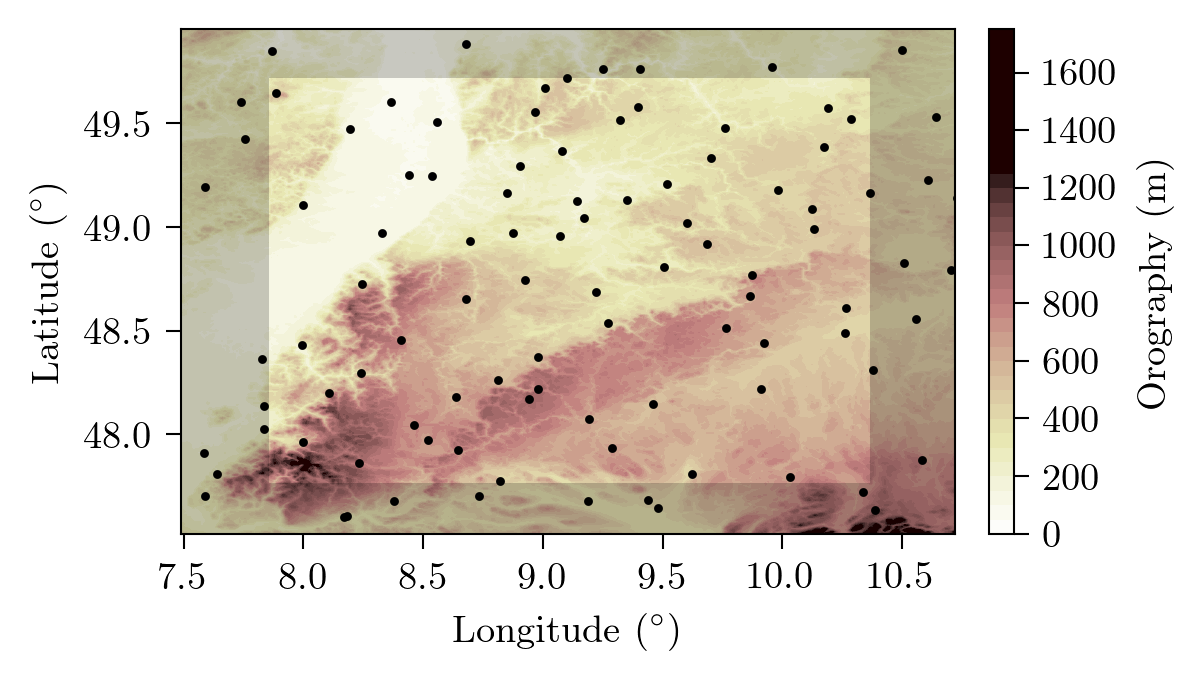
\includegraphics[width=0.48\textwidth]{figures/fig_02_orography.png}
	\caption{
		Model orography extracted from the used CLM input files \citep{european_environment_agency_digital_2013}.
		The model orography is based on the European digital elevation model.
		The black points are representing the 99 measurement sites, used for synthetic observations of the 2-metre-temperature.
		The black shaded boundary region is not used in figures with area means.
	}
	\label{fig:model_orography}
\end{figure}

\subsection{Data assimilation}

We combine a background forecast $\textbf{x}^{\text{b}}$ with observations $\mathbf{y}^\text{o}$ in data assimilation to get an analysed state $\textbf{x}^{\text{a}}$, which should be as close as possible to an unknown true state $\textbf{x}^{\text{t}}$.
Both, background forecast and observations, are a disturbed representation of the true state with the identity mapping and a possibly non-linear observation operator $H(\mathbf{x})$ as mapping operators, respectively.
Both have presumably additive Gaussian errors $\mathbf{\epsilon}^\text{b}$ and $\mathbf{\epsilon}^\text{o}$ with error covariances $\textbf{B}$ and $\textbf{R}$, respectively,
\begin{align}
	\mathbf{x}^\text{b} &= \mathbf{x}^\text{t} + \mathbf{\epsilon}^\text{b}, & \mathbf{\epsilon}^\text{b} \sim \mathcal{N}(\mathbf{0}, \mathbf{B}),\label{eq:formulation_kf_back}\\
	\mathbf{y}^\text{o} &= H(\mathbf{x}^\text{t}) + \mathbf{\epsilon}^\text{o}, & \mathbf{\epsilon}^\text{o} \sim \mathcal{N}(\mathbf{0}, \mathbf{R}).
	\label{eq:formulation_kf_obsop}
\end{align}

Based on this Gaussian assumption, we can represent the analysed state as linear combination between the observations and background forecast with $\mathbf{H}^{T}$ as linearized and transposed observation operator \citep{kalman_new_1960,kalnay_atmospheric_2003},
\begin{equation}
	\mathbf{x}^\text{a} = \mathbf{x}^\text{b} + \mathbf{B}\mathbf{H}^{T}(\mathbf{H}\mathbf{B}\mathbf{H}^{T} + \mathbf{R})^{-1} (\mathbf{y}^\text{o} - H(\mathbf{x}^\text{b})).\label{eq:formulation_kalman_filter}
\end{equation}

We parametrize the observational error covariance $\mathbf{R} = (\sigma^\text{o})^2 \mathbf{I}$ as diagonal matrix with an observational standard deviation $\sigma^\text{o} = 0.1\,\text{K}$, which is static in time and constant across all observations.
To solve Eq. \eqref{eq:formulation_kalman_filter}, we need a background forecast $\mathbf{x}^\text{b}$, the background error covariance $\mathbf{B}$, and a linearized observation operator $\mathbf{H}$.
We compare in this study two different ways to define these matrices, the Simplified Extended Kalman filter (SEKF) and an Ensemble Kalman filter (EnKF).
In the following, we will shortly describe these schemes.

\subsubsection{Simplified Extended Kalman filter}

We use a deterministic background forecast for the SEKF.
This background forecast is updated at 00:00 UTC based on grid-point observations at 12:00 UTC and Eq. \eqref{eq:formulation_kalman_filter}.
In the SEKF, we only update the soil moisture.
To derive $\mathbf{H}$, which describes the sensitivity of 2-metre-temperature observations to perturbations in soil moisture, we perturb the soil moisture for a finite differences' approximation as described in \citet{hess_assimilation_2001,rosnay_simplified_2013}.
To create the finite differences' approximation, we need only one additional perturbed model run for every soil layer because CLM has a column-based soil model.
The background error covariance $\mathbf{B} = (\sigma^\text{b})^2 \mathbf{I}$ is assumed to be diagonal and static in time with $\sigma^\text{b} = 0.01\,\text{m}^3 \text{m}^{-3}$ as standard deviation.

\subsubsection{Ensemble Kalman filter}

Ensemble Kalman filters are based on a Monte-Carlo approximation of the background state $\mathbf{x}^\text{b}$ and the background covariance $\mathbf{B}$, based on $n$ ensemble members and with $\mathbf{x}^{\prime\text{b}}_{i}=\mathbf{x}^\text{b}_{i} - \overline{\mathbf{x}}^\text{b}$ as ensemble perturbations of the $i$-th ensemble member,
\begin{align}
	\mathbf{x}^\text{b} \approx \overline{\mathbf{x}}^\text{b} &=
	\frac{1}{n}\sum_{i=1}^{n} \mathbf{x}^\text{b}_{i},\label{eq:ens_approx_mean}\\
	\mathbf{B} &=
	\frac{1}{n-1}\sum_{i=1}^{n} (\mathbf{x}^\text{b}_{i} - \overline{\mathbf{x}}^\text{b})(\mathbf{x}^\text{b}_{i} - \overline{\mathbf{x}}^\text{b})^{T}\label{eq:ens_approx_cov}\\
	&= \frac{1}{n-1}\sum_{i=1}^{n} \mathbf{x}^{\prime\text{b}}_{i} (\mathbf{x}^{\prime\text{b}}_{i})^{T}.\nonumber
\end{align}
With this ensemble approximation, we can update the background state by Eq. \eqref{eq:formulation_kalman_filter} and obtain a mean analysis state $\overline{\mathbf{x}}^\text{a}$, which represents the most probable analysis state at time $t$.
This analysis state is then a weighted linear combination of the background ensemble members $\mathbf{x}^\text{b}_{i}$.
We use an implementation of the Localized Ensemble Transform Kalman Filter (LETKF, \citet{bishop_adaptive_2001,hunt_efficient_2007}) in this study, where this weighting is explicitly represented with a column-wise matrix of all background perturbations $\mathbf{X}^{\prime\text{b}}$ and the mean ensemble weights $\overline{\textbf{w}}$,
\begin{equation}
	\overline{\mathbf{x}}^\text{a} = \overline{\mathbf{x}}^\text{b} + \mathbf{X}^{\prime\text{b}} \overline{\mathbf{w}}.\label{eq:letkf_eq}
\end{equation}
These mean ensemble weights are then estimated with Eq. \eqref{eq:formulation_kalman_filter} in the space spanned by the ensemble perturbations $\mathbf{X}^{\prime\text{b}}$.
To derive a linearized observation operator for Eq. \eqref{eq:formulation_kalman_filter}, each ensemble member is independently transformed into observational space, and afterwards, the observation operator is linearized around the ensemble mean in observational space $H(\mathbf{x}^{\text{b}}) \approx \frac{1}{n}\sum_{i=1}^{n} H(\mathbf{x}^{\text{b}}_{i})$.

The increments for every ensemble member are obtained based on the mean ensemble weights and a deterministic and symmetric square-root filter with $\mathbf{w}^\prime_{i}$ as additional perturbative member weights for the $i$-th ensemble member,
\begin{equation*}
	\mathbf{x}^\text{a}_{i} = \overline{\mathbf{x}}^\text{b} + \mathbf{X}^{\prime\text{b}} (\overline{\mathbf{w}}+\mathbf{w}^\prime_{i}).
\end{equation*}

In our experiments, we use the same model configuration for our nature run as for our data assimilation experiments.
These experiments are thus model-error-free compared to the nature run.
Nevertheless, the ensemble approximations from Eq. \eqref{eq:ens_approx_mean} and Eq. \eqref{eq:ens_approx_cov} induce sampling errors.
Because of these sampling errors, we include in our EnKF multiplicative prior covariance inflation as described in \citet{hunt_efficient_2007}.

The number of ensemble members is low compared to the state dimensions, especially for data assimilation across compartments.
This discrepancy in the dimensionality introduces spurious correlations into the background covariances \citep{miyoshi_10240-member_2014}, which can degrade the analysis.
To reduce spurious correlations, the LETKF utilizes observational localization.
We base our horizontal and vertical localization scheme on Gaspari-Cohn weighing functions \citep{gaspari_construction_1999}, which are also used for operational data assimilation in the atmosphere \citep{schraff_kilometre-scale_2016}.


\section{Experiments}

In this section, we will describe our experiments.
First, we will explain our experimentation strategy.
Secondly, we will shortly characterize the weather and soil conditions within our nature run.

\subsection{Experimentation strategy}

In our experiments, we create an ensemble to investigate interactions between temperature in the atmospheric boundary layer and soil moisture.
Our experiments are based on a perfect model assumption such that we use the same model configuration for every run, depicted in Table \ref{tab:model_config}.
The model configuration for the atmosphere is almost the same as for the COSMO-DE setup that was in operational use at the DWD until 2018, except that we use a smaller area.
The model area is based on the Neckar catchment in Baden-Württemberg and spans a region of $\sim 300\,\text{km}$ in latitudinal direction and $\sim 280\,\text{km}$ in longitudinal direction as shown in Figure \ref{fig:model_orography}.

\begin{table}[h]
	\caption{General framework configuration\label{tab:model_config}}
	\begin{tabular}{l|l}
		Variable & Value \\ 
		\hline 
		Atmospheric model & COSMO 4.21 \\
		Horizontal resolution & $\sim 2.8\,\text{km}$\\
		Grid points & Lat: $109$, Lon: $99$\\
		Vertical levels & $50$\\
		\hline
		Soil model & CLM 3.5\\
		Horizontal resolution & $\sim 1\,\text{km}$\\
		Grid points & Lat: $302$, Lon: $267$\\
		Vertical levels & $10$\\
		\hline
		Data assimilation & LETKF + SEKF\\
		Inflation & Prior mult. inflation ($\gamma = 1.006$)\\
		Hori. localization & Gaspari-Cohn ($15\,\text{km}$)\\
		Vert. localization & Atmosphere: GC ($0.3\,\ln\,\text{hPa}$)\\
		& Soil: GC ($0.7\,\text{m}$)\\
		Available observations & $99$\\
		Observational error & $0.1\,\text{K}$		
	\end{tabular}
\end{table}

Our data assimilation framework \citep{finn_py_bacy_2020, finn_torch-assimilate_2020} is developed in Python \citep{van_rossum_python_1995}, PyTorch \citep{paszke_pytorch_2019}, Xarray \citep{hoyer_xarray_2017}, and Dask \citep{dask_development_team_dask_2016,rocklin_dask_2015}.
This framework is coupled to TerrSysMP by files such that the background and first guess are read-in as output files from the models.
The analysis is then based on input files to restart the forecast models.\\

We define a nature run (NATURE) as our truth in this study and to get our 2-metre-temperature observations.
We generate hourly 2-metre-temperature fields by using the diagnostic COSMO 2-metre-temperature output. For the observations, we select $99$ grid points (marked as black dots in Figure \ref{fig:model_orography}), given by the nearest horizontal neighbour grid point to real measurement sites.
To introduce an observational error, we add to these selected observations independent and identically distributed (i.i.d.) unbiased Gaussian noise with a standard deviation of $\sigma^\text{o} = 0.1\,\text{K}$.

Since COSMO is a limited-area model, we have to define for the experiments lateral boundary conditions, besides initial conditions.
In all experiments, including the nature run, we use the same lateral boundary conditions in the atmosphere.
The lateral boundary conditions are generated based on the $18$-th member of the COSMO-DE EPS ensemble from the DWD with the same horizontal and vertical resolution as our model setup.
Accordingly, we do not induce any model perturbations by the lateral boundary conditions.
Our only perturbations in the atmosphere and soil are a result of initial soil moisture and soil temperature perturbations.

A single run with a similar model configuration and a spin-up of $6$ years builds the foundation for our initial conditions in the atmosphere and soil.
Every run has the same initial conditions in the atmosphere, whereas we perturb the initial soil conditions by correlated Gaussian perturbations similar to \cite{schraff_kilometre-scale_2016}.
As horizontal correlation function, we use a truncated Gaussian kernel with a standard deviation of 14 grid points ($\approx 14 \,\text{km}$) and a truncation radius of 42 grid points.
The same type of truncated Gaussian correlation is used in vertical dimensions with a standard deviation of $0.5\,\text{m}$ and a truncation after $1\,\text{m}$.
For soil moisture perturbations, we perturb the soil moisture saturation, which is the volumetric soil moisture scaled by the saturation point, and we further restrict that the resulting saturation lies between $0$ and $1$.
We use unbiased Gaussian noise with a standard deviation of $0.06$ for the soil moisture saturation and $1\,\text{K}$ for the soil temperature across all layers.

Based on these initial soil perturbations, we generate $40$ ensemble members for our ensemble experiments.
We initialize our nature run with the initial conditions of a hypothetical $41$-th ensemble member to make sure that the ensemble spread within an open-loop run is representative for the error of its ensemble mean to the nature run.
The deterministic run for the SEKF experiment is initialized with the ensemble mean of the $40$ different ensemble members to get comparable results between the LETKF and SEKF.

We start the model runs for all of our experiments at 2015-07-30 00:00 UTC.
The first $36$ hours of simulation are used as spin-up such that perturbations can propagate from the soil into the atmosphere.
After this spin-up phase, starting at 2015-07-31 12:00 UTC, we start with our six different experiments.
The models are restarted because of our file-based data assimilation, and processes in the turbulent kinetic energy scheme are reset, which can be seen as some kind of model error.
To mitigate this possible model error source, we will restart after 2015-07-31 12:00 UTC all model runs hourly.
We will simulate a period of one week (seven days) and finish our experiments at 2017-08-07 18:00 UTC.
We will shortly describe the experiments in the following; their abbreviations are given in Table \ref{tab:exp_desc}.\\

\begin{table*}[ht]
	\caption{
		Experiment abbreviations with experiment description about the run type, assimilation scheme and which variables are updated\label{tab:exp_desc}
	}
	\begin{tabular}{l|l|l|l|l}
		Experiment name & run type & scheme & updated variable & description\\
		\hline
		NATURE & deterministic & - & - & Reference run\\
		ENS & ensemble (40) & - & - & Open-loop ensemble\\
		LETKF Soil & ensemble (40) & LETKF & soil moisture & weakly-coupled EnKF\\
		LETKF Soil + Temp & ensemble (40) & LETKF & soil moisture + atmospheric temperature & strongly-coupled EnKF\\
		DET & deterministic & - & - & Open-loop deterministic\\
		SEKF & deterministic & SEKF & soil moisture & weakly-coupled SEKF
	\end{tabular}
\end{table*}

An open-loop ensemble forecast without data assimilation (ENS) is used as comparison for the scores in section \ref{sec:results} and to investigate the evolution of the ensemble spread with regard to initial ensemble perturbations.
Starting from this open-loop ensemble at 2015-07-31 12:00 UTC, we run an experiment, where we assimilate the 2-metre-temperature with a LETKF to update the soil moisture only (LETKF Soil).
This setting can be seen as weakly-coupled data assimilation experiment and is mainly used as comparison to the SEKF.
We enforce the non-negativity of the soil moisture analysis by clipping negative values after the assimilation to zero.
We expect that most of the soil-generated perturbations in the atmospheric boundary layer can be found in the atmospheric boundary layer temperature.
Based on this expectation, we additionally update the atmospheric temperature together with the soil moisture in the LETKF Soil+Temp experiment.
We cast this experiment as baseline experiment for strongly-coupled data assimilation, and we will extensively evaluate this experiment in the second part of the results.

In another experiment, we run an open-loop deterministic forecast without data assimilation (DET).
This deterministic forecast is initialized with the same initial values as the ensemble mean.
We expect that the errors of this deterministic forecast are comparable to the open-loop ensemble mean.
This deterministic run acts then as baseline experiment for the SEKF experiment, where we assimilate grid-point based the 2-metre-temperature at 12:00 UTC into the soil moisture at 00:00 UTC, the night before.
Normally, an optimal interpolation scheme is used to generate the grid-point-based screen-level observations, which would introduce additional errors into the comparison between LETKF and SEKF.
We simplify in this study our grid-point based observations for the SEKF.
We map the 2-metre-temperature of the NATURE run from the COSMO grid to the CLM grid by bilinear interpolation, as done in the OASIS coupler.
This interpolated field is then perturbed by i.i.d. unbiased Gaussian noise with a standard deviation of $\sigma^\text{o} = 0.1\,\text{K}$.
With this standard deviation, the observational errors for the SEKF are similar to the observational errors for the LETKF.
Because the SEKF is a smoothing algorithm, we already make use of the pseudo-observations at 2015-07-31 12:00 and start our SEKF experiment at 2015-07-31 00:00.

In data assimilation experiments, the direct and accumulated assimilation impact is difficult to quantify as each experiment evolves along its own trajectory.
To disentangle effects of different approximations on the direct assimilation impact without accumulated increments, we make additional offline data assimilation experiments.
In these offline data assimilation experiments, we generate analyses based on the trajectories of the SEKF and the LETKF Soil+Temp experiment without restarting the model system; the background forecasts of these offline experiments are therefore the same as for the SEKF and the LETKF Soil+Temp experiment, respectively.
Into these existing background trajectories, we assimilate observations from the NATURE run with different approximations.

\begin{figure}
	%\centering
	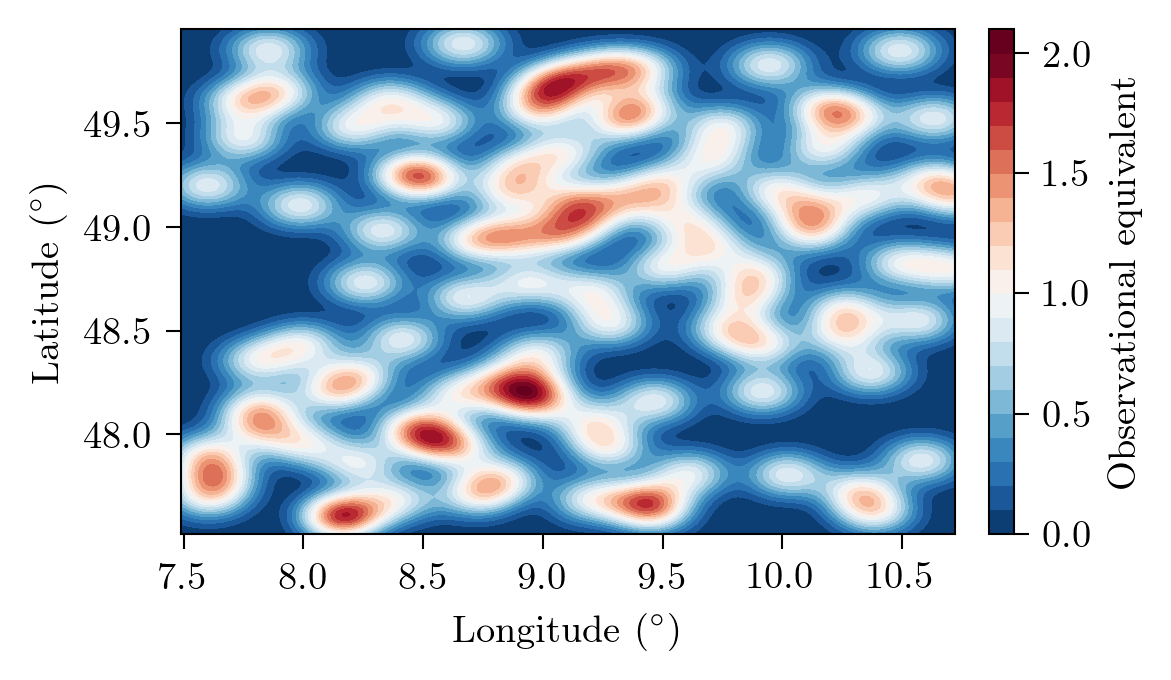
\includegraphics[width=0.48\textwidth]{figures/fig_01_obs_equivalent.png}
	\caption{
		Number of potential observational equivalents per grid point estimated based on the chosen horizontal and vertical localisation radius in soil (see Table \ref{tab:model_config}), representative for $0.21\,\text{m}$ depth.
		Blue colours characterize fewer equivalents per grid point compared to grid-point-based assimilation (e.g. SEKF), whereas red colours indicate more equivalents.
	}
	\label{fig:obs_equivalent}
\end{figure}

For our ensemble-based LETKF experiment, we have to define additional localization radii and an inflation factor.
We choose here a horizontal localization radius of $15\,\text{km}$, which is quite small in comparison to operationally used values in the atmosphere (between $50\,\text{km}$ and $100\,\text{km}$, \citealt{schraff_kilometre-scale_2016}).
This small radius represents smaller error-covariance length-scales for the land surface and atmospheric boundary layer compared to typical error length-scales in the free atmosphere.
In the atmosphere, we localize vertically in terms of logarithmic pressure and use a typical value ($0.3\,\ln\text{hPa}$), which is also used in operational settings \citep{schraff_kilometre-scale_2016}.
Observations in the atmospheric boundary layer have their largest impact on soil moisture analysis at root-depth \citep{munozsabater_assimilation_2019}, while afterwards the physically explainable impact is negligible.
Our vertical localization radius in soil is therefore chosen ($0.7\,\text{m}$) such that the innovations for soil levels below the root-depth ($5$-th layer) are dampened.
Because the impact of observations is additive, we can sum up the localization weights and estimate the here so-called potential observational equivalents (Figure \ref{fig:obs_equivalent}).
These equivalents tell us how many observations are potentially available per grid point, if we neglect involved ensemble sensitivities, in comparison to a fully-observed field with a one-dimensional assimilation scheme.
The mean observational equivalent for the $5$-th soil layer ($0.21\,\text{m}$ depth) is $0.566$, indicating that we have roughly half the number of potential observations per grid-point relative to a fully-observed field.
We have thus only a limited observability within the LETKF experiments, and in some areas, we would expect no assimilation impact at all.
We additionally set the multiplicative prior covariance inflation factor to $1.006$, which reflects that we have only sampling errors and no model error.

\subsection{Weather and soil conditions}

\begin{figure}
	%\centering
	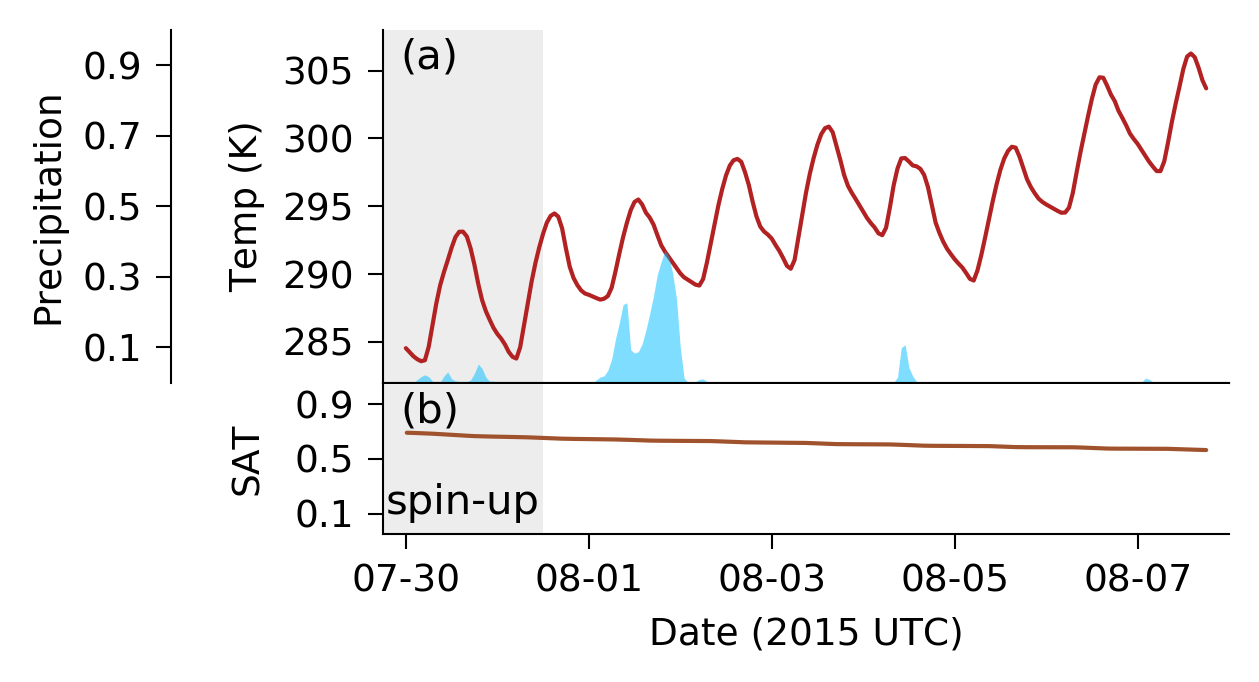
\includegraphics[width=0.48\textwidth]{figures/fig_03_overview.png}
	\caption{
		Mean weather overview over the simulated time period, extracted from the NATURE run.
		The grey-shaded area indicates the spin-up phase, which is not used for the experiments.
		(a) The hourly development of the 10 metre temperature as area mean, while the blue bars show the percentage of grid points with precipitation ($> 0\,\text{kg}\,\text{m}^{-2}\,\text{h}^{-1}$) in the previous hour.
		(b) Hourly soil moisture saturation in root-depth ($0.21\,\text{m}$ depth) as area mean.
	}
	\label{fig:test_case_overview}
\end{figure}

The daily mean 2-metre-temperature increases with time in our seven-day simulation period, whereas the soil moisture in root-depth decreases (Figure \ref{fig:test_case_overview}).
The soil is in a mixed soil moisture regime, as indicated by saturation values around $0.5$.
The amplitude of the diurnal cycle in the 2-metre-temperature is further quite large.
Together with the soil moisture drying and the temperature increase, this amplitude indicates a period with strong solar irradiance and without large precipitation events.
The only larger precipitation event is on 2015-08-01, while a smaller event on 2015-08-04 has the largest impact on the 2-metre-temperature.
Based on this weather overview only, we would expect a coupling between atmospheric boundary layer temperature and soil moisture in root-depth during day-time.
We can therefore say that we expect some data assimilation impact on the soil moisture by assimilating the 2-metre-temperature.


\section{Results}\label{sec:results}

We structure this section into two general parts.
In the first subsection, we will compare our experiments and show what we can learn from this comparison.
Afterwards, we analyse the LETKF Soil+Temp experiment more in detail with regard to driving factors in the assimilation.\\

We can expect that assimilating the 2-metre-temperature into soil moisture improves the forecast of the atmospheric boundary layer (e.g. \citet{carrera_assimilation_2019}). 
We will analyse in a first step the impact of data assimilation into soil moisture on the prognostic boundary layer temperature (Figure \ref{fig:err_t_long}) in $10\,\text{m}$ height above ground, the lowest prognostic model level.

\begin{figure*}[ht]
	%\centering
	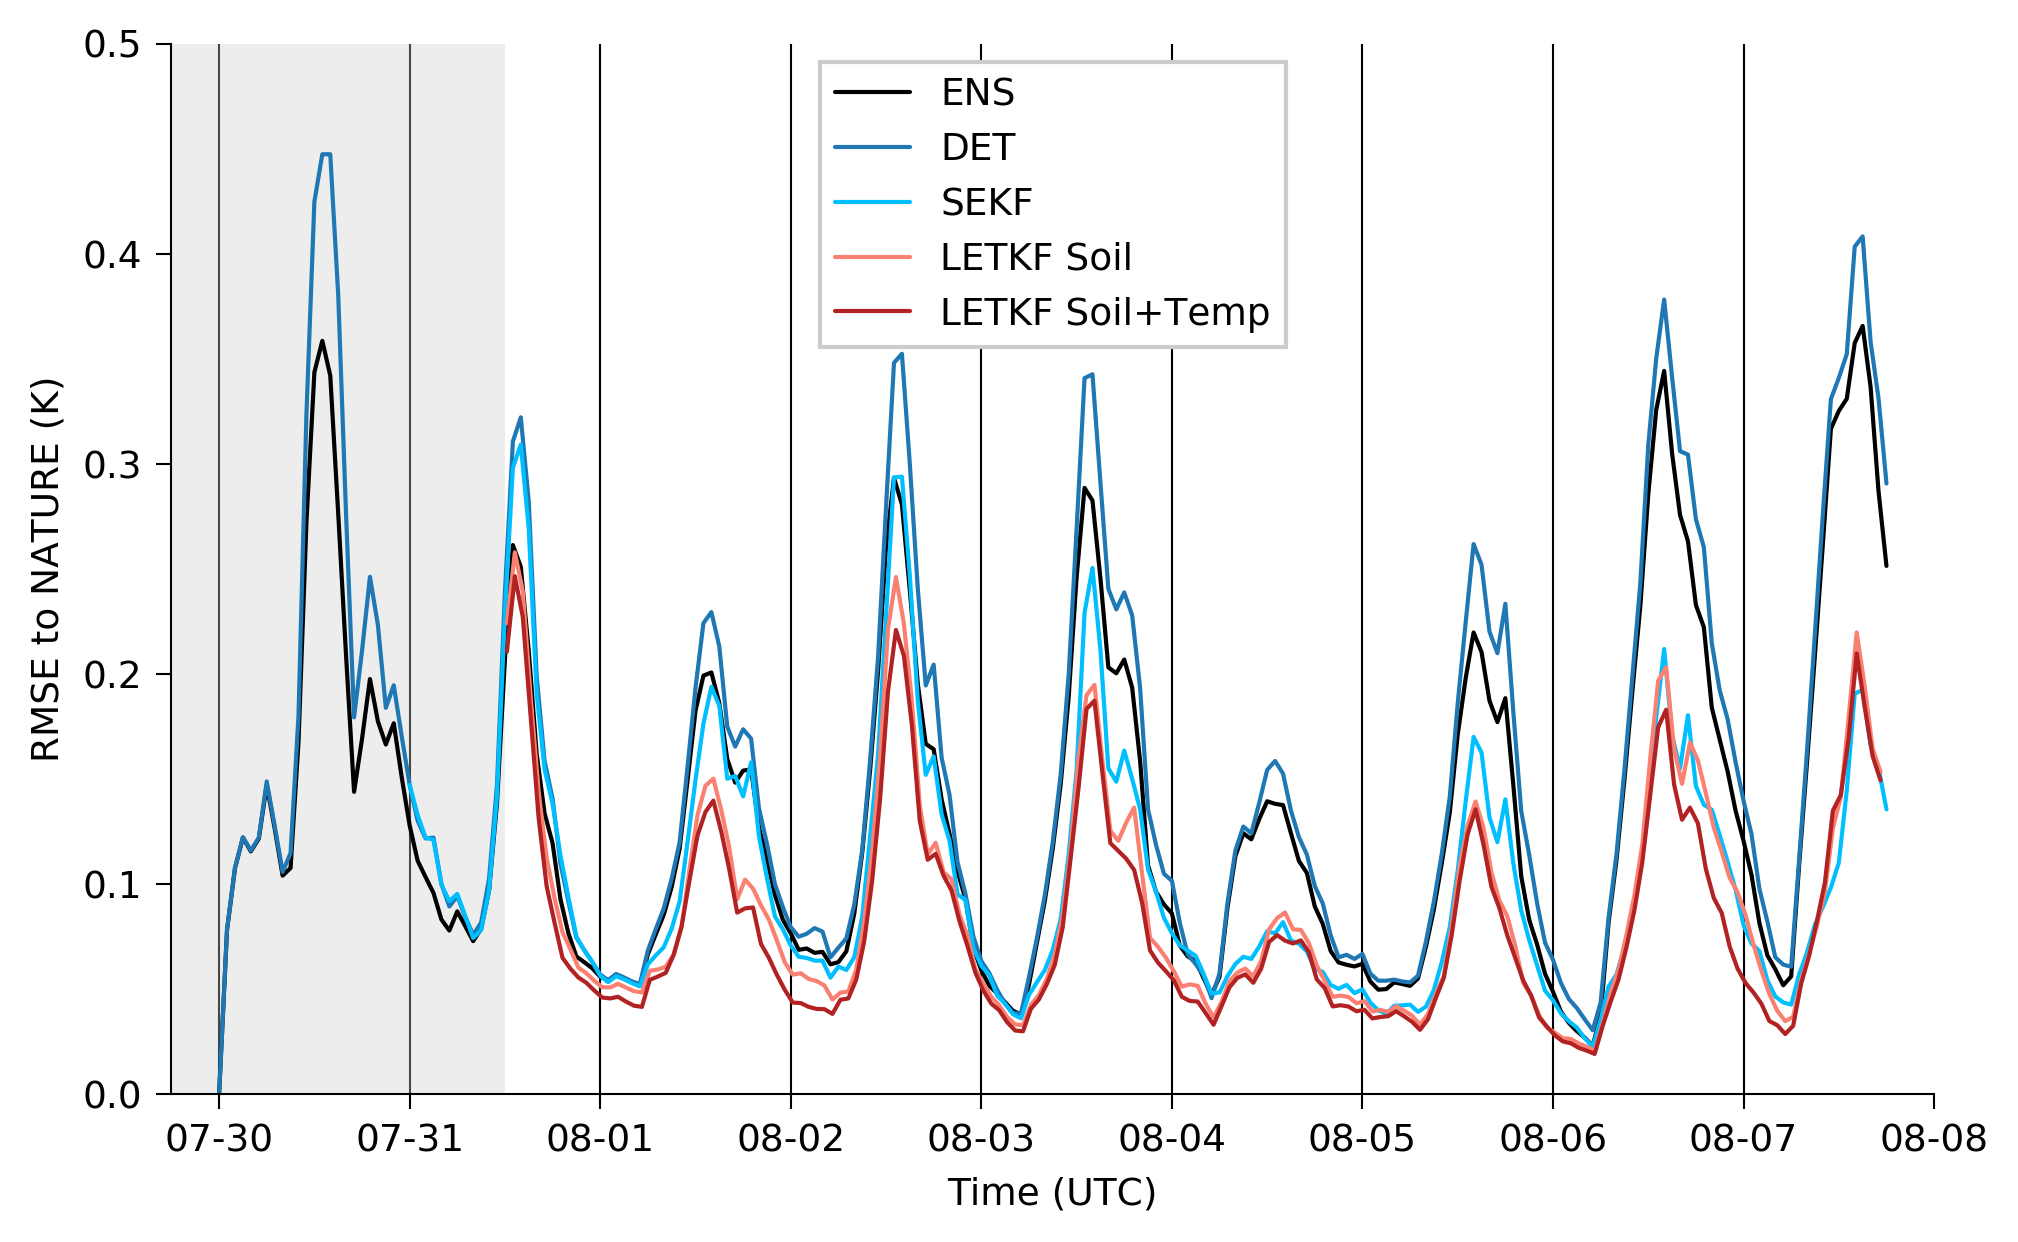
\includegraphics[width=\textwidth]{figures/fig_04_err_t_long.png}
	\caption{
		RMSE and ensemble spread of different experiments for temperature in 10 metres height as area mean relative to the RMSE of ENS.
		Different colours denote different experiments.
		The red colours indicate LETKF experiments with an ensemble, while the bluish colours represent experiments based on a deterministic run.
		All solid lines show the RMSE, while the red dashed line is the mean ensemble spread over all grid points.
		The grey-shaded region is the spin-up phase.
	}
	\label{fig:err_t_long}
\end{figure*}

Every data assimilation experiment (SEKF; LETKF Soil; LETKF Soil+Temp) has a substantially lower Root-Mean-Squared-Error (RMSE) to NATURE than their counterpart without data assimilation (DET; ENS, Table \ref{tab:exp_rmse}).
Because this result is found throughout the experiments, this improvement is independent of additional updates in the atmospheric boundary layer.
This result confirms previous studies that updating the soil moisture with 2-metre-temperature observations has a positive assimilation impact on the forecast of the atmospheric boundary layer.

\begin{table}[ht]
	\caption{
		Spatial and temporal root-mean squared error for depicted experiments compared to NATURE with hourly data from 2015-07-31 13:00Z to 2017-08-07 18:00Z, representing the background trajectory of the experiments.\label{tab:exp_rmse}
	}
	\begin{tabular}{l|c|c}
		Name & T2m (K) & H2O ($\text{m}^3 \text{m}^{-3}$)\\
		\hline
		ENS & 0.158 & 0.0169 \\
		LETKF Soil & 0.105 & 0.0114 \\
		LETKF Soil + Temp & 0.098 & 0.0112 \\
		DET & 0.178 & 0.0171 \\
		SEKF & 0.118 & 0.0145
	\end{tabular}
\end{table}

All experiments have a clearly defined diurnal cycle in the RMSE with the highest errors during day-time.
We find the same diurnal cycle in the data assimilation impacts with the highest impacts during day-time and only small impacts during night.
Perturbations within the atmosphere are only a result of initial soil perturbations or data assimilation, because our lateral boundary conditions are the same for every run.
During day-time, the coupling between land surface and atmospheric boundary layer propagates perturbations into the atmosphere, whereas these two compartments are decoupled during night-time. 
The collapse of the atmospheric boundary layer in the evening leads to a strong decrease of the atmospheric perturbations.
Due to this process, collected information by data assimilation from the day before is also partially lost.

The LETKF Soil+Temp experiment has the smallest error of all experiments, indicating a small positive impact of additionally updating the atmospheric temperature.
Nudging the atmospheric temperature to the observations helps us to reduce error components related to a drift of trajectories compared to the NATURE run.
By construction of the experiment, the largest part of errors are nevertheless soil-induced, which limits the additional impact of updating the atmospheric temperature.
We additionally have a loss of information due to the collapsing boundary layer, as discussed before, and the differences between the LETKF Soil and the LETKF Soil+Temp experiment remain small over the simulation window.

The assimilation impact of the SEKF experiment is similar to the impact of the LETKF Soil experiment, despite the fact that the latter experiment has a smaller absolute magnitude of error.
Because the same decreased error can be noticed between the DET and ENS experiment, the smaller errors of the LETKF Soil experiment are mainly accountable to the difference in the type of experiment.
Based on this result, both data assimilation methods, the SEKF and LETKF, are similar effective in reducing errors in the atmospheric boundary layer temperature by updating the soil moisture only.\\

\begin{figure*}[ht]
	%\centering
	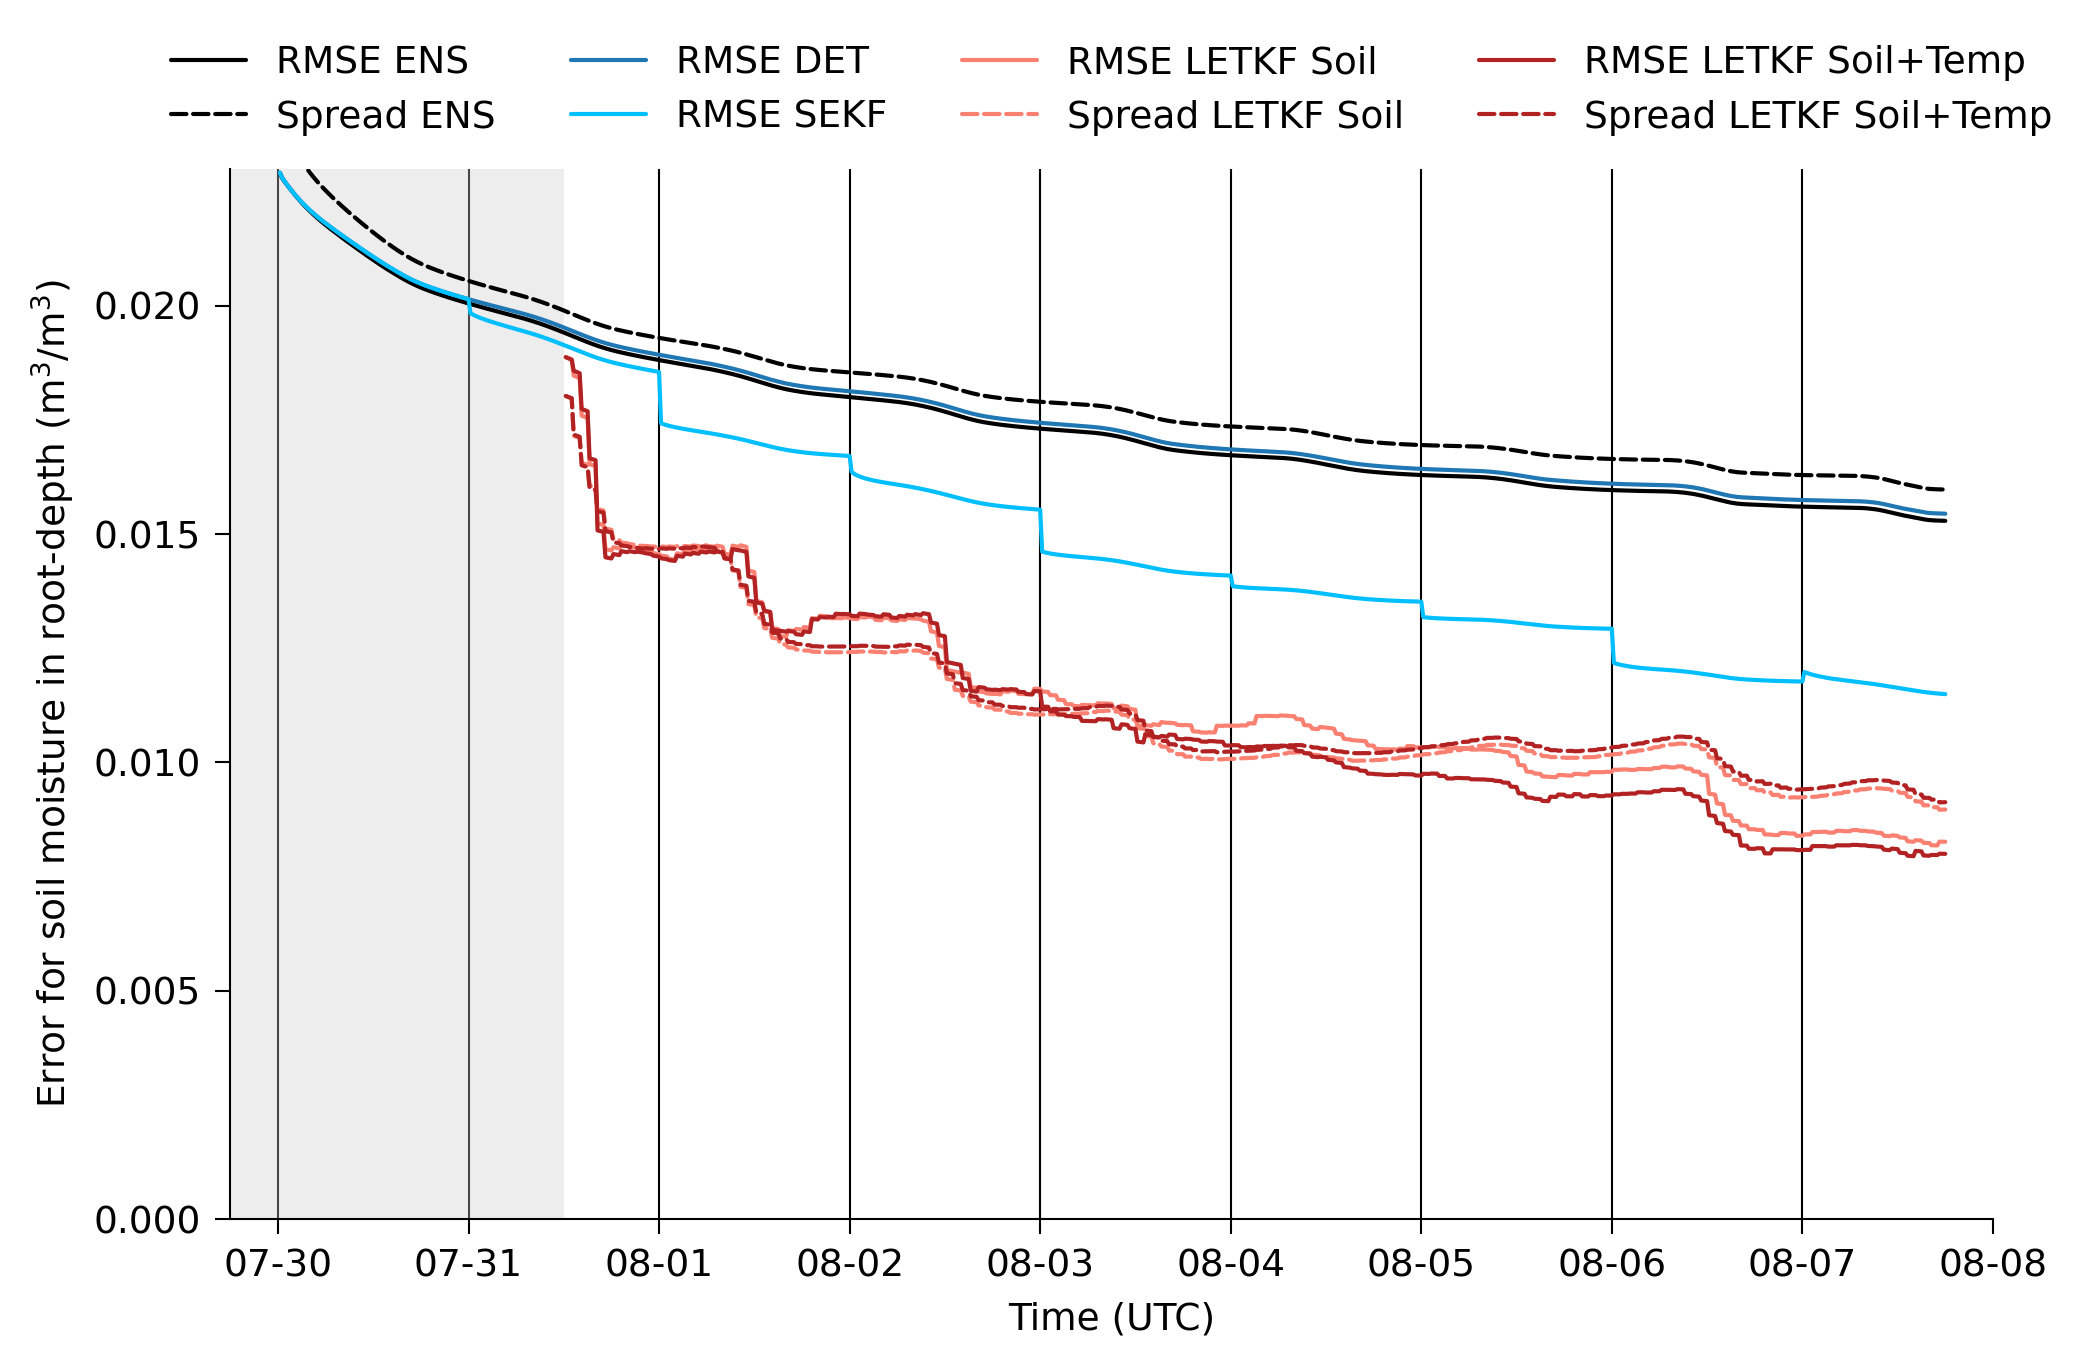
\includegraphics[width=\textwidth]{figures/fig_05_err_h2o_long.png}
	\caption{
		RMSE and ensemble spread of different experiments for soil moisture in root-depth as area mean.
		Different colours denote different experiments.
		The red colours indicate LETKF experiments with an ensemble, while the bluish colours represent experiments based on a deterministic run.
		All solid lines show the RMSE, while the red dashed line is the mean ensemble spread over all grid points.
		The greyish shaded region is the spin-up phase, where no data assimilation experiment was run.
	}
	\label{fig:err_h2o_long}
\end{figure*}

We can expect that the assimilation of 2-metre-temperature observations into soil moisture has also a positive impact on the soil moisture in root-depth, if we improve the forecast of the boundary layer temperature based on the coupling between atmosphere and land.
The error of all experiments reduces with time as the soil dries out in the simulation period (Figure \ref{fig:err_h2o_long})
Furthermore, data assimilation decreases the error in the SEKF, LETKF Soil, and LETKF Soil+Temp experiment compared to their corresponding reference experiments (DET; ENS).
The positive assimilation impact in the LETKF experiment is a result of corrections during day-time, whereas a neutral assimilation impact prevails at night.
This diurnal cycle in the impact again reflects the relevance of the coupling strength between land surface and atmosphere, and the flow-dependent background error covariances of the LETKF can represent the situation- and time-dependent coupling strength.
The LETKF is therefore able to improve the soil moisture analysis by hourly data assimilation.

The LETKF Soil experiment has a smaller error than the SEKF experiment, but they have similar impacts on the boundary layer temperature.
This increased impact in soil moisture is a result of filtering instead smoothing, used in the SEKF experiments.
The SEKF can correct foreseeable errors at noon in advance, whereas we only correct instantaneous errors in the filtering framework.
Smoothing has thus an advantage compared to filtering for correcting errors in the atmospheric boundary layer based on updates of the soil moisture.
For soil moisture, the information content of a single update step is limited by the coupling strength.
Hence, hourly updating the soil moisture with the LETKF is capable to extract more information from limited observations than the SEKF with a fully-observed field and a single update step per day.

Additional nudging of the simulated boundary layer temperature towards the observed temperature results in a positive impact in the LETKF Soil+Temp experiment compared to the LETKF Soil experiment.
By updating the boundary layer temperature, we increase the consistency in the analysis errors, which has also a positive assimilation impact on later cycles.
In soil, this positive assimilation impact is accumulated over time, and the error of the LETKF Soil+Temp experiment is further reduced in comparison to the LETKF Soil experiment.\\

Up to this point, we only looked into the error development of either the temperature at the lowest atmosphere layer or the soil moisture in root-depth as spatial mean.
In the following, we will analyse how the assimilation impact is spatial distributed (Figure \ref{fig:spatial_impact}) in the LETKF Soil and SEKF experiment.

\begin{figure*}[ht]
	%\centering
	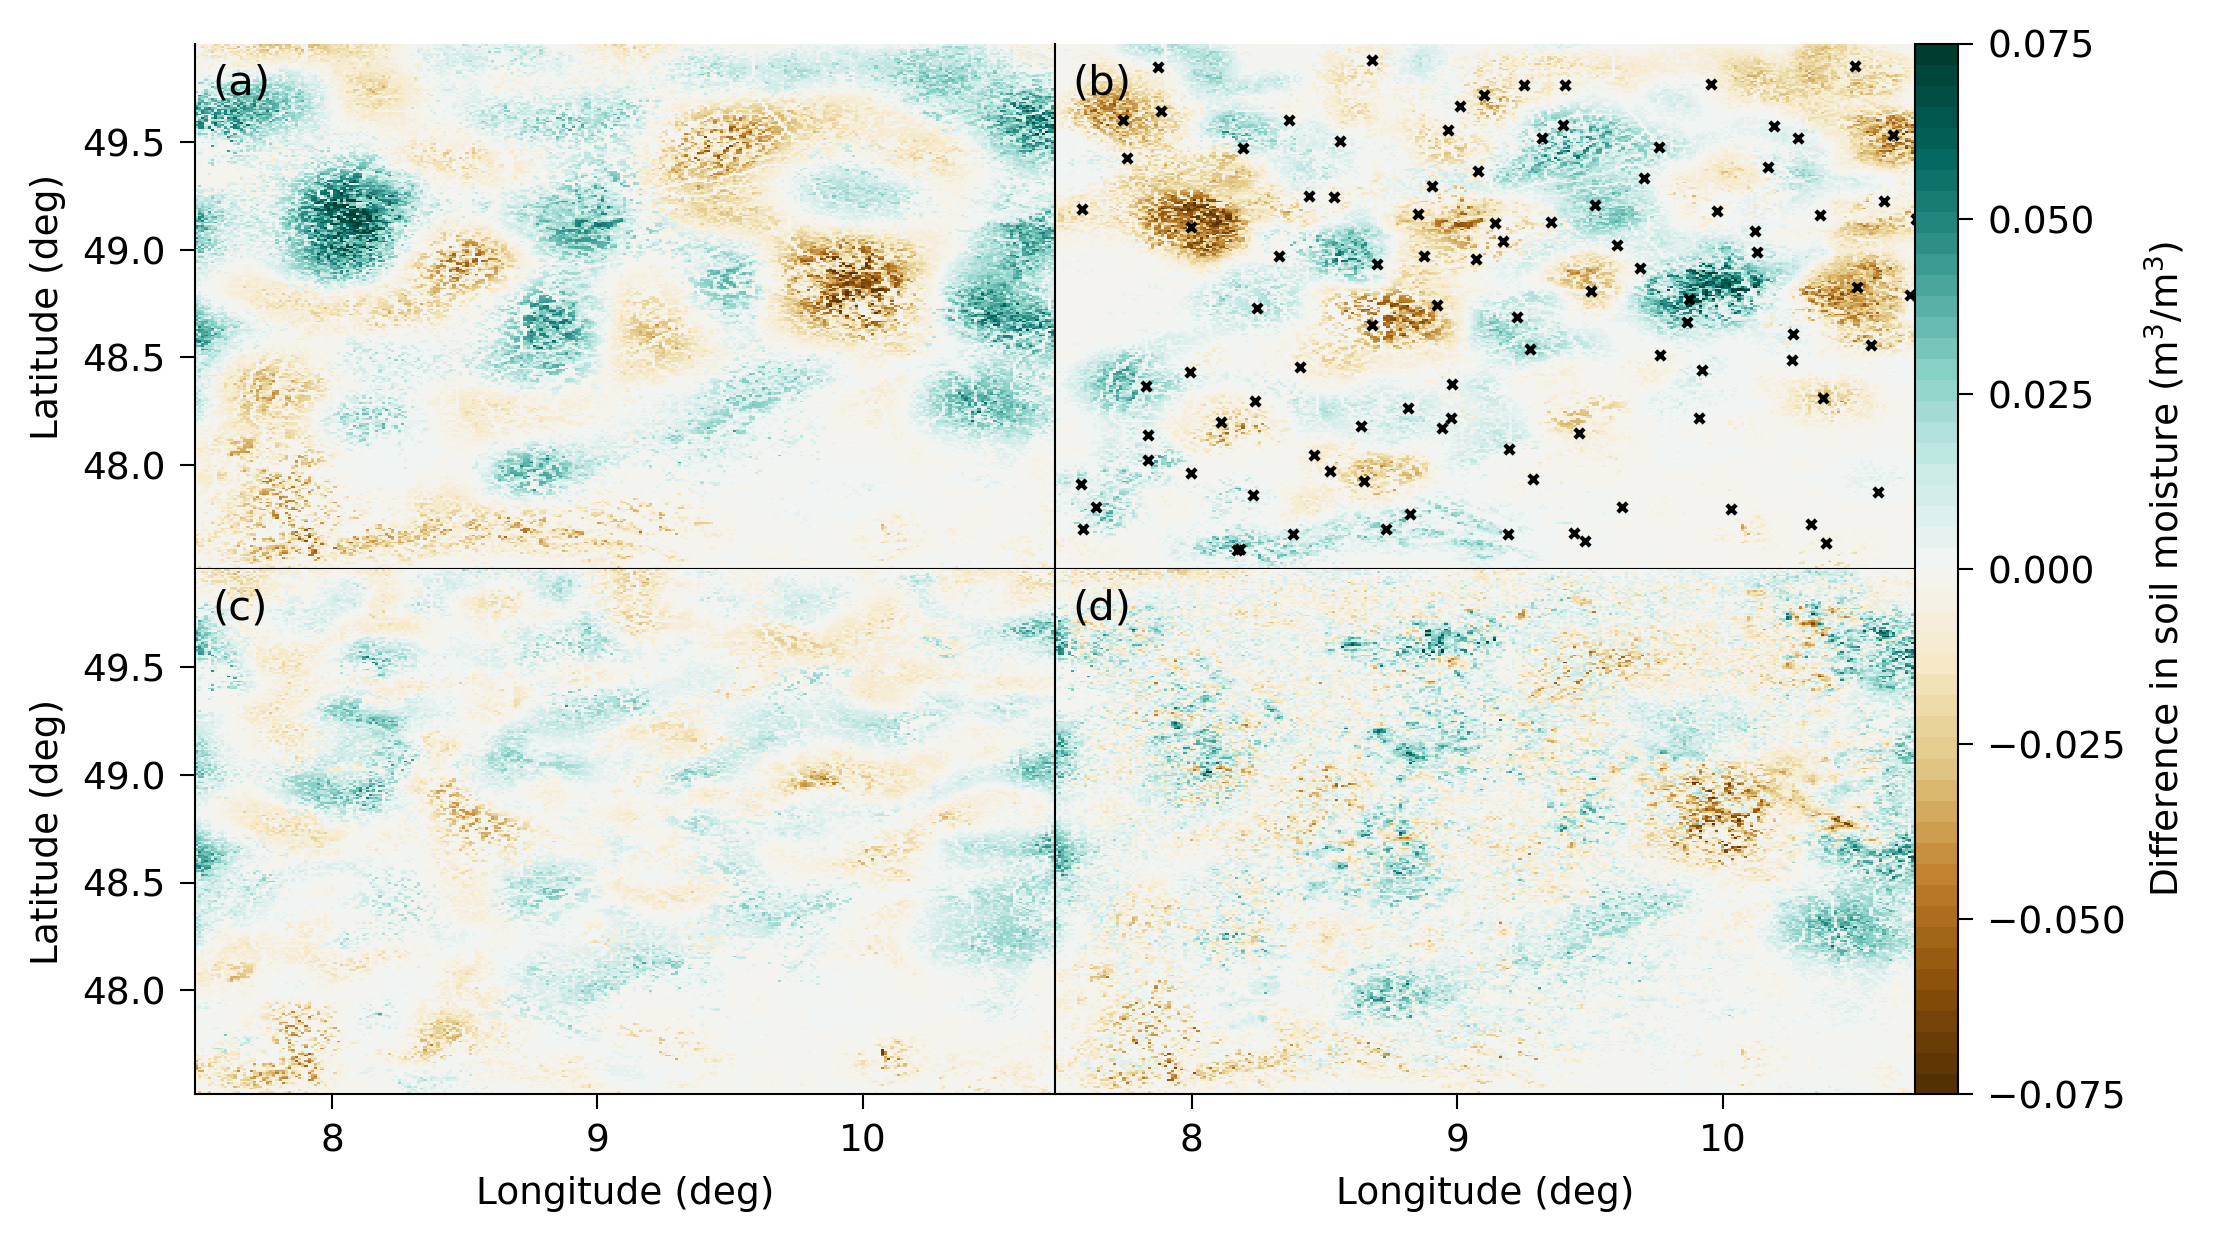
\includegraphics{figures/fig_06_spatial_impact.png}
	\caption{
		Spatial impact of data assimilation in the ensemble and deterministic experiments at the last time step.
		The upper panels show the error of the ENS experiment (ensemble mean, a) to the NATURE run and the increment of the LETKF Soil (ensemble mean, b) to the ENS (ensemble mean) experiment.
		The lower panels are the error of the LETKF Soil (ensemble mean, c) and the SEKF (d) experiment to the NATURE run.
		Blue colours indicate a positive difference, whereas brown colours represent a negative difference.
		The black crosses in (b) indicate the observational positions as in Figure \ref{fig:model_orography}.
	}
	\label{fig:spatial_impact}
\end{figure*}


The spatial distribution of the error in the ENS experiment (Figure \ref{fig:spatial_impact}, a) compared to the NATURE run is caused by the initialization of the experiments.
Processes leading to a change in patterns within the soil moisture act on longer time-scales than our seven-day simulation time, especially in time periods without large precipitation events.
Our initial errors, induced by correlated Gaussian fields, thus determine the amplitude and patch size of the errors in the experiments without data assimilation.

Data assimilation of the 2-metre-temperature corrects the initial errors, as shown in the accumulated increment of the LETKF Soil experiment compared to the ENS experiment (Figure \ref{fig:spatial_impact}, b).
This increment depends not only on the error size, but also on the observational positions and chosen localization radius.
Nevertheless, the amplitude and patch size of the increments have a similar order of magnitude as the errors, showing that the number of observations and horizontal localization radius are enough and well tuned, respectively.

These increments also influence the remaining error of the LETKF Soil experiment compared to the NATURE run (Figure \ref{fig:spatial_impact}, c).
Errors are especially dampened in this experiment, if observational position and initial condition errors match.
The construction of the ensemble perturbations \citep{hunt_efficient_2007} and spatial localization in the LETKF lead to a spatial smoother error field than for the SEKF experiment (Figure \ref{fig:spatial_impact}, d).
The SEKF experiment has also higher error amplitudes than the LETKF Soil experiments, showing the effectiveness of the LETKF in this case.
Furthermore, the one-dimensional approximation in the SEKF results in error fluctuations across a small area, which are not apparent in the errors and LETKF Soil experiment.
The LETKF Soil experiment has thus a spatially more balanced and higher impact than the SEKF experiment, especially in the eastern part of the domain.\\

In the following (Figure \ref{fig:offline_exp}), we will show the RMSE for soil moisture in root-depth of the offline experiments based on the SEKF trajectory (Figure \ref{fig:offline_exp}, a) and on the LETKF Soil+Temp trajectory (Figure \ref{fig:offline_exp}, b).

\begin{figure*}[ht]
	%\centering
	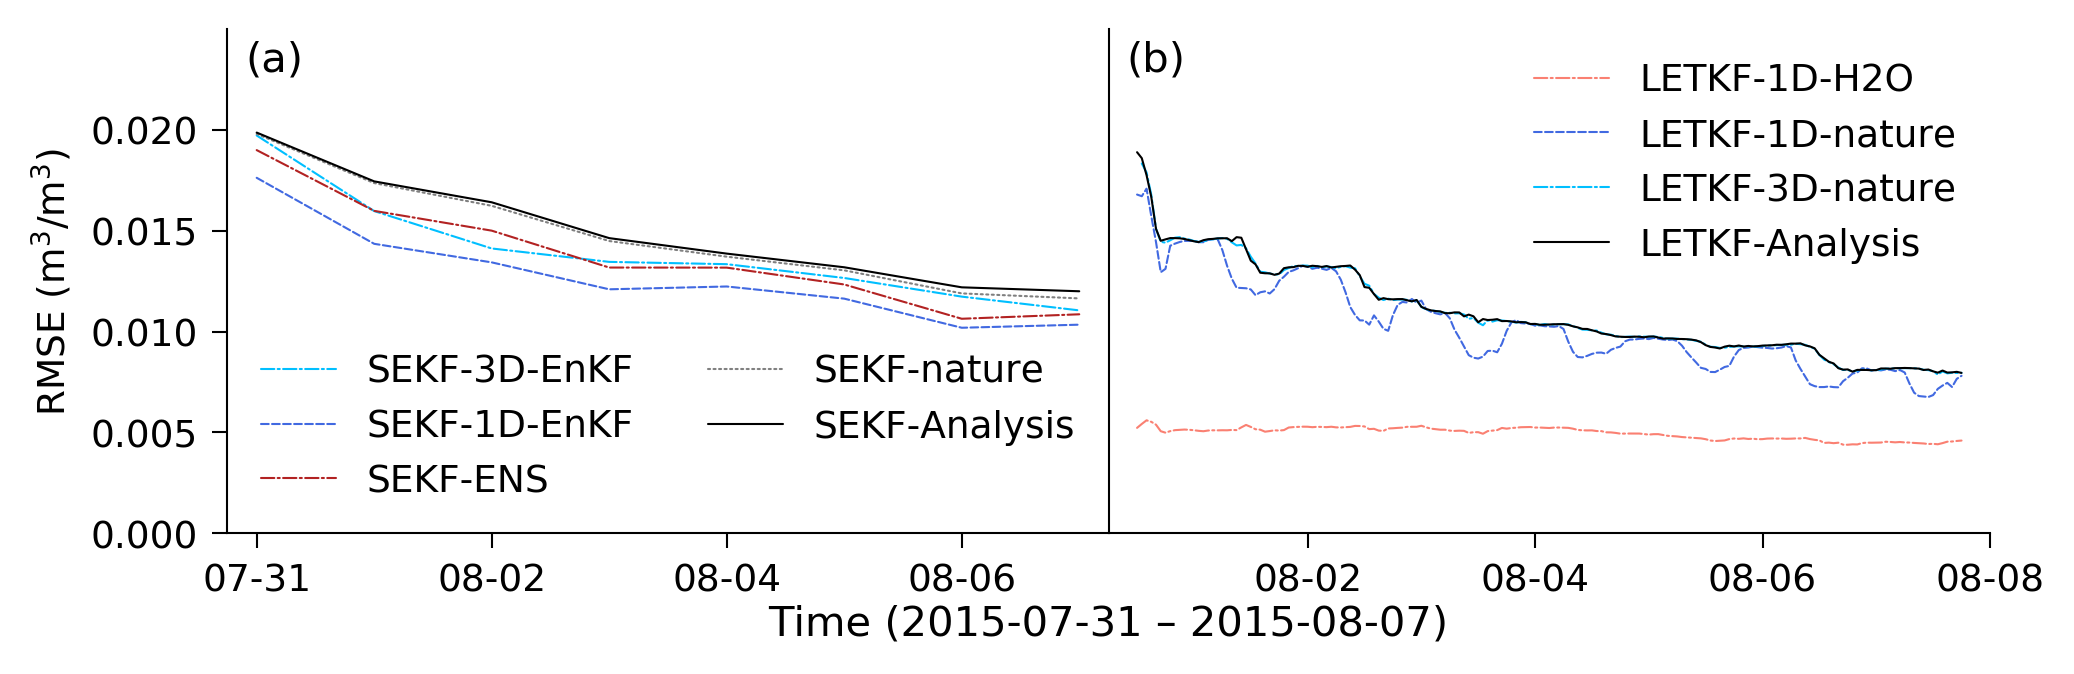
\includegraphics{figures/fig_07_offline_exp.png}
	\caption{
		RMSE of offline data assimilation experiments for soil moisture in root-depth based on (a) the SEKF and (b) the LETKF Soil+Temp background trajectory.
		Blueish colours indicate an assimilation of 2-metre-temperature observations from the NATURE run with an ensemble Kalman filter and without observation error, whereas the soil moisture is directly assimilated in the salmon-coloured 1D-H2O experiment in b).
		The original analyses are black and the SEKF analysis based on perfect NATURE run observations greyish dotted.
		Only the ensemble mean was updated in column-based 1D EnKF experiments, whereas a full LETKF was used in the 3D EnKF experiments.
	}
	\label{fig:offline_exp}
\end{figure*}

The comparison between an experiment with perfect observations, extracted from the NATURE run, and disturbed observations allows us to get an impact of the random observational error.
For the SEKF base trajectory (Figure \ref{fig:offline_exp}, a), the difference between an offline experiment with observations from the NATURE run, denoted SEKF-nature, and the original analyses is small.
Based on these marginal differences, random observational errors have only a negligible impact on the errors of the SEKF trajectory.

In the SEKF-ENS experiment, we replace the finite-differences' approximation for the Jacobians in Eq. \eqref{eq:formulation_kalman_filter} by an ensemble approximation from the ENS experiment.
We make here the assumption that the ENS experiment is like an external ensemble data assimilation cycle with constrained perturbations in the atmosphere, since we use the same lateral boundary conditions in all experiments.
This offline experiment thus resembles the current SEKF implementation at the ECMWF \citep{ecmwf_ifs_2019}, except the fact that we do not restart the trajectory within this offline experiment.
The error compared to SEKF-nature is reduced, indicating that the ensemble approximation stabilizes the Jacobians in comparison to the finite-differences' approximation.

We take dynamic background covariances from the ENS experiment into account in the SEKF-1D-EnKF experiment, where we use an EnKF instead of a SEKF.
In this experiment, we further reduce the error compared to the SEKF-ENS experiment.
This error reduction has two reasons:
On one hand, we have dynamic covariances, which resemble the flow-dependent uncertainties.
On the other hand, the ensemble spread of ENS experiment is larger than the analysis error of the SEKF experiment and the static background covariances for the SEKF.
We thus overestimate the assimilation impact in the SEKF-1D-EnKF experiment, which is then a lower bound for the SEKF error.

We replace the column-based data assimilation with a LETKF-based assimilation of $99$ discrete observation points in the SEKF-3D-EnKF experiment.
Here, we assimilate with a LETKF, based on the perturbations from the ENS experiment, observations from the NATURE run at 12:00Z into the background trajectory of the SEKF experiment at 00:00Z.
This increases the analysis error compared to the SEKF-1D-EnKF experiment, because we have only limited observations compared to a fully observed field.
Nevertheless, the error of the SEKF-3D-EnKF experiment is smaller than the SEKF-nature, showing that the ensemble-based assimilation is preferable to a finite-differences-based SEKF.

Similar results can be seen in the offline data assimilation experiments based on the LETKF Soil+Temp experiment (Figure \ref{fig:offline_exp}, b).
Replacing the disturbed observations with perfect observations in the LETKF-3D-nature analyses has almost no impact on the analyses error.
Using a fully-observed field in the LETKF-1D-nature reduces the error compared to the LETKF-3D-nature experiment, similar to the error reduction in the SEKF experiments.
Nevertheless, the impact of a fully-observed field is low compared to the accumulated error reduction in the LETKF Soil+Temp experiment.
The LETKF thus assimilates effectively limited boundary layer observations across the atmosphere-land inferface.

We directly assimilate the soil moisture in root-depth in the LETKF-1D-H2O experiment.
With this direct assimilation, we deactivate the source of uncertainty within the vertical covariances, translating from 2-metre-temperature to soil moisture in root-depth.
The margin between LETKF-1D-H2O and LETKF-1D-nature is thus representative for the assimilation impact associated to the coupling between atmosphere and land.
Based on this margin, the coupling between the 2-metre-temperature and soil moisture dominantly controls the assimilation impact on soil moisture, also during day-time.\\

The sensible heat flux acts as main coupler between soil moisture and 2-metre-temperature, whereas the evapotranspiration has a bigger impact on humidity in the atmosphere.
Based on these physical considerations, we will now show the dependency of the sensible heat flux on the soil moisture (Figure \ref{fig:sensible_smi}).

\begin{figure}[ht]
	%\centering
	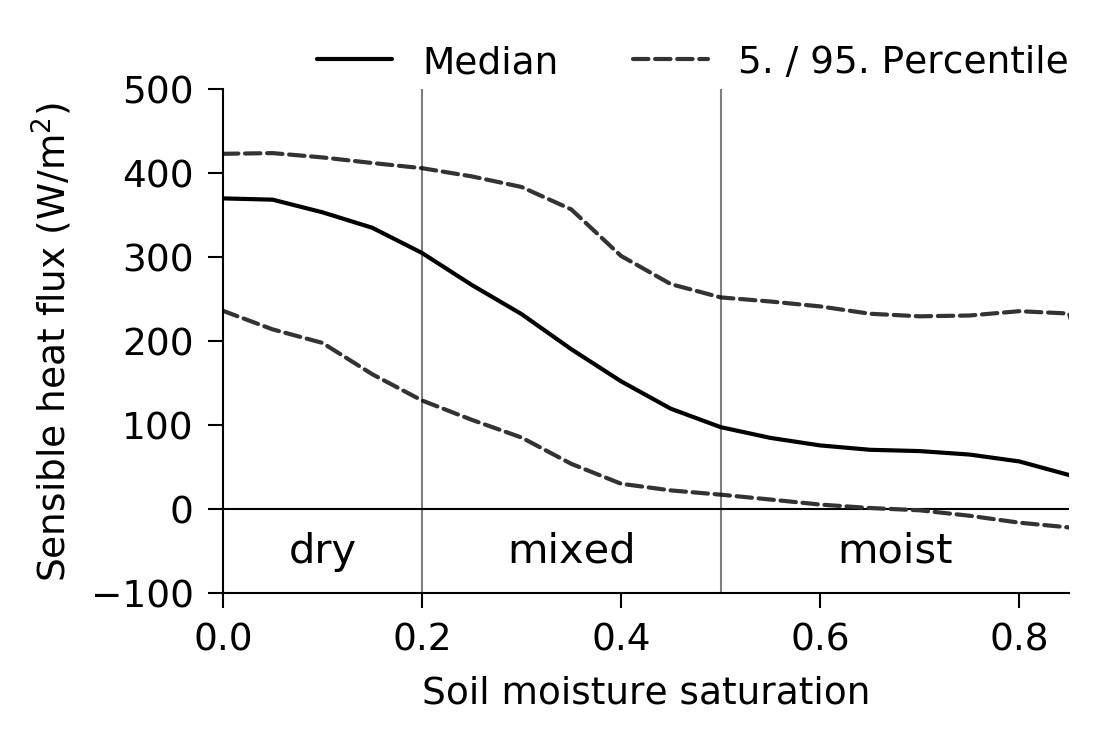
\includegraphics[width=0.48\textwidth]{figures/fig_08_sensible_sat.png}
	\caption{
		The sensible heat flux in dependence on the root-depth soil moisture saturation at 14:00Z.
		All values are estimated based on all ensemble members in the LETKF Soil+Temp experiment, all grid points and all days between 2015-07-31 to 2015-08-07 for 14:00Z.
		The black line is the median over the binarised heat flux ($\Delta\text{SAT} = 0.05$), whereas the dotted lines shown the 5. and 95. percentile.
	}
	\label{fig:sensible_smi}
\end{figure}

Based on the non-linear dependency of the sensible heat flux on the soil moisture (Figure \ref{fig:sensible_smi}), we can expect different assimilation impacts for different soil moisture regimes.
The sensible heat flux reaches its maximum values in the dry regime, where the ensemble mean soil moisture saturation is below $0.2$.
Here, near the wilting point, changes in soil moisture have only a small impact on the sensible heat flux, because there is nevertheless to little moisture for plants and their evapotranspiration.
The same insensitivity can be found in the moist regime, where the ensemble mean saturation is above $0.5$.
Plants have in this regime enough water for transpiration and the sensible heat flux is almost insensitive to changes in soil moisture.
Hence, the sensible heat flux value is more influenced by other factor, as indicated by higher variances across a soil moisture bin, and we expect here the smallest assimilation impact.
In the mixed regime, where the saturation is between $0.2$ and $0.5$, plants regulate  their transpiration based on the soil moisture, leading to higher sensitivities in the sensible heat flux to changes in the soil moisture.
We would therefore expect that most available information from the 2-metre-temperature for the soil moisture is encoded within this mixed regime.\\

In Figure \ref{fig:h_impact}, we classify the soil moisture with these three regimes to show its influence on the potential assimilation impact in soil moisture itself.
Based on the LETKF-1D-nature experiment from Figure \ref{fig:offline_exp}, we use a potential assimilation impact, which would be the assimilation impact on the soil moisture in root-depth, if we would observe the whole 2-metre-temperature NATURE field.
We define here the potential assimilation impact as the difference in the area mean RMSE  to the NATURE run from the analysis of the LETKF-1D-nature experiment to the background of the LETKF Soil+Temp experiment for soil moisture.

\begin{figure}[ht]
	%\centering
	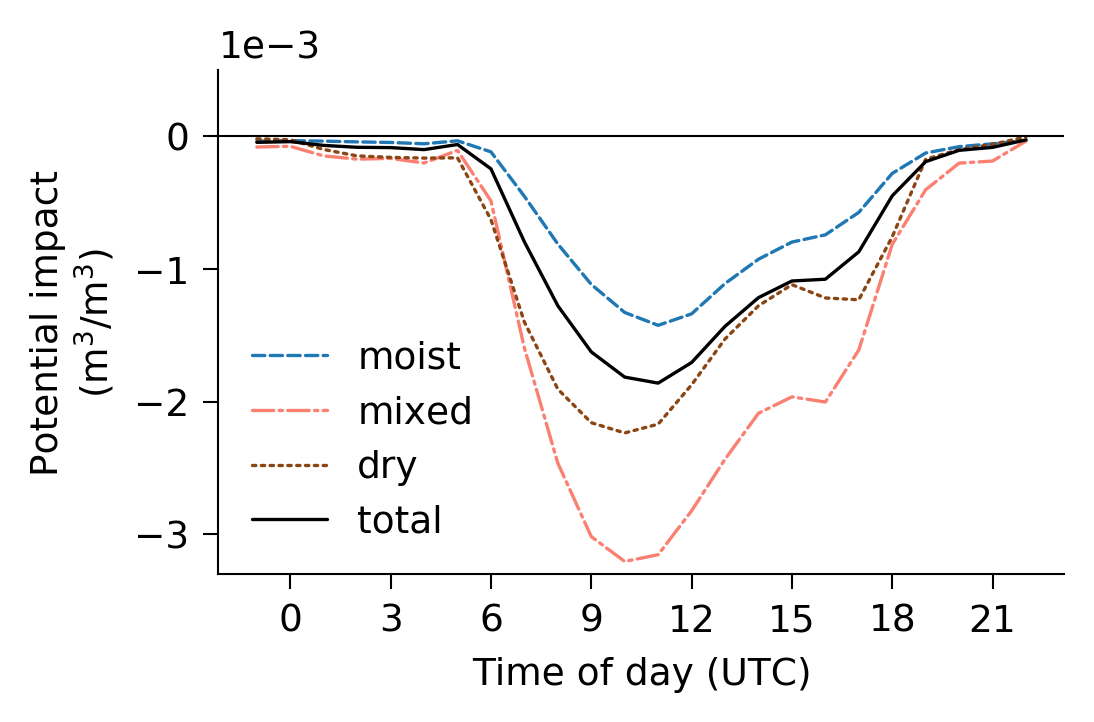
\includegraphics[width=0.48\textwidth]{figures/fig_09_soil_moisture_impact.png}
	\caption{
		Area mean diurnal cycles for the potential assimilation impact, valid from 2015-07-31 19:00Z to 2015-08-07 18:00Z.
		We have a positive assimilation impact for negative values and vice versa.
		The grid point are classified based on the soil moisture saturation classes in Figure \ref{fig:sensible_smi} and the background ensemble mean soil moisture saturation.
	}
	\label{fig:h_impact}
\end{figure}

The soil moisture saturation clearly determines the potential assimilation impact (Figure \ref{fig:h_impact}), as previously expected.
We find the highest potential impact in grid points with mixed regime, where the sensible heat flux has the highest sensitivity to changes in the soil moisture.
The assimilation has its lowest impact in the moist regime, because the sensible heat flux has here its least sensitivity to changes in soil moisture and is mostly influenced by other factors.
For our seven-day simulation, we conclude that the soil moisture itself is a main factor to explain variabilities in the assimilation impact across grid points.

In all regimes, we have a positive assimilation impact during day-time, whereas a negligible impact during night.
The solar irradiance is the main driver for the coupling between atmospheric boundary layer and land surface and shapes also the diurnal cycle of the assimilation impact.
Nevertheless, in the late afternoon the potential impact deviates from its expected diurnal cycle, which cannot be explained by solar irradiance alone.
This potential impact deviation indicates a mechanism, which reinforces the positive assimilation impact in the late afternoon.

In the following, we will reveal that the coupling is additionally controlled by the temporal development of the atmospheric boundary layer (Figure \ref{fig:cycle_corr}), leading to the deviation in the late afternoon.
We analyse this temporal development within the LETKF Soil+Temp experiment.

\begin{figure}[ht]
	%\centering
	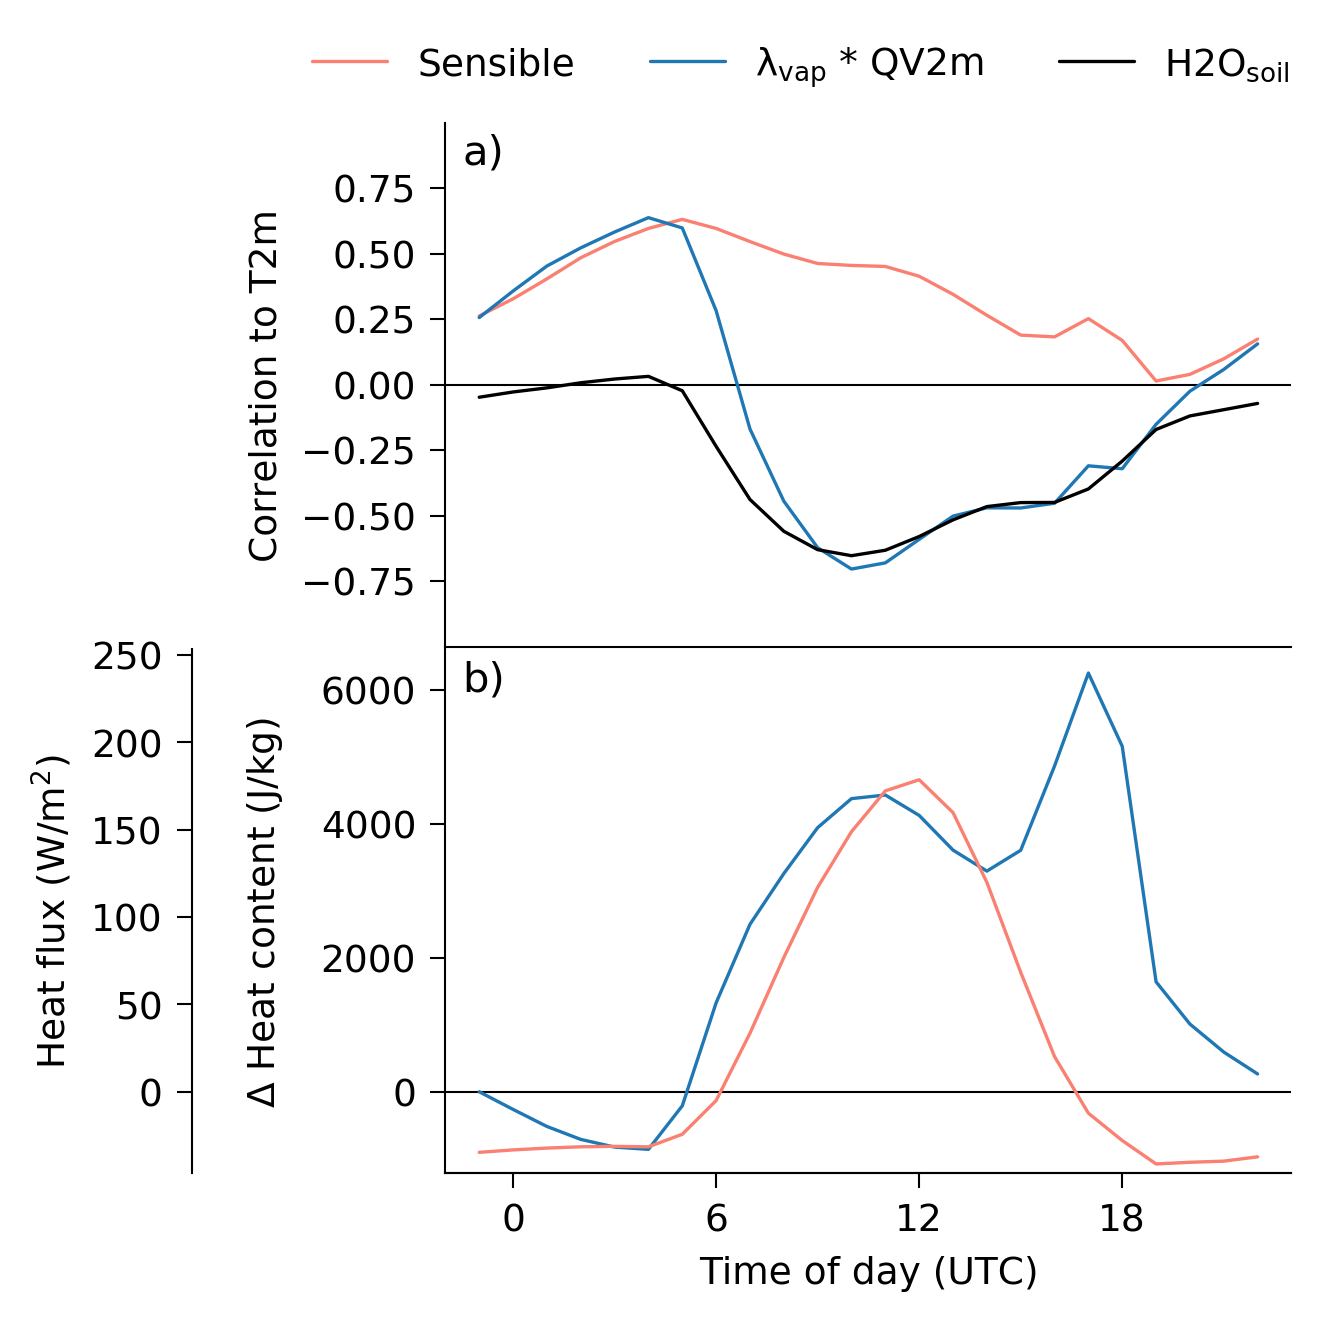
\includegraphics[width=0.48\textwidth]{figures/fig_10_cycle_corr.png}
	\caption{
		Area mean diurnal cycles for: a) the ensemble correlations for different variables (sensible heat flux, water vapour heat content in humidity in 2 metre height, and soil moisture) to the 2-metre-temperature in the LETKF Soil+Temp experiment; b) Change of the heat content relative to 23:00Z for the heat content in humidity, and the sensible heat flux, in the LETKF Soil+Temp experiment as average over all ensemble members, valid for 2015-07-31 19:00Z to 2015-08-07 18:00Z. The water vapour heat content is estimated based on a constant latent heat of vaporization $\lambda_{\text{vap}} = 2.501 \times 10^6\, \text{J}\, \text{kg}^{-1}$ and the specific humidity in 2 metre height.
	}
	\label{fig:cycle_corr}
\end{figure}

As main driver for the assimilation impact, the coupling between land surface and atmosphere correlates the soil moisture to the 2-metre-temperature (Figure \ref{fig:cycle_corr}, a).
Driven by this coupling, perturbations in the 2-metre-temperature accumulate during day-time.
This accumulation decreases the impact of the coupler – the sensible heat flux – on the 2-metre-temperature perturbations, which decorrelates the sensible heat flux and the 2-metre-temperature with time.
The water vapour content in the lower boundary layer is mainly controlled by evapotranspiration, and thus, negatively correlated to the 2-metre-temperature during day-time.
At night, an increased water vapour content in the atmosphere decreases the radiative cooling of the land surface \citep{harrison_effect_1981}, which results in a positive correlation to the 2-metre-temperature.
After sunrise, and before perturbations in the boundary layer are accumulated, the sensible heat flux has a direct impact on the 2-metre-temperature.

The same reinforcement mechanism, as in the potential assimilation impact,
can be found in the correlations of the sensible heat flux and soil moisture to the 2-metre-temperature.
The sensible heat flux follows nevertheless a diurnal cycle without any additional peak (Figure \ref{fig:cycle_corr}, b).
In contrast to this diurnal cycle, the reinforcement mechanism also heavily influences the diurnal cycle of the water vapour content.
Based on this fact, we can trace the reason of the reinforcement mechanism back to the growth and collapse of the boundary layer.
The land surface heats up with increasing solar irradiance in the morning.
With time, the sensible heat flux and evapotranspiration transport the heat into the boundary layer \citep{stull_introduction_1988}, causing an increase in the heat content of the boundary layer.
In the afternoon, the solar irradiance decreases again with time such that also differences between boundary layer and land surface decrease, resulting in lower heat fluxes.
Together with a growth of the mixed boundary layer, these lower heat fluxes cause a decrease in the heat content few meters above the surface, as seen in the water vapour content.
As a consequence of the strong decrease in solar irradiance, the near-surface boundary layer collapses into a thin strongly-stratified boundary layer.
Propagated heat is now stored within this thin layer, leading to a rapid increase in the heat content.
This rapidly increased heat content then also strengthens the atmosphere-land coupling above the land surface in the late afternoon.\\

The atmosphere-land coupling controls the information content encoded within the vertical covariances.
In the following, we will also take horizontal covariances and the impact of localization into account and take a deeper look into the dependence of the diagonal covariance on the horizontal distance between 2-metre-temperature and soil moisture (Figure \ref{fig:covariance_dist}).

\begin{figure}[ht]
	%\centering
	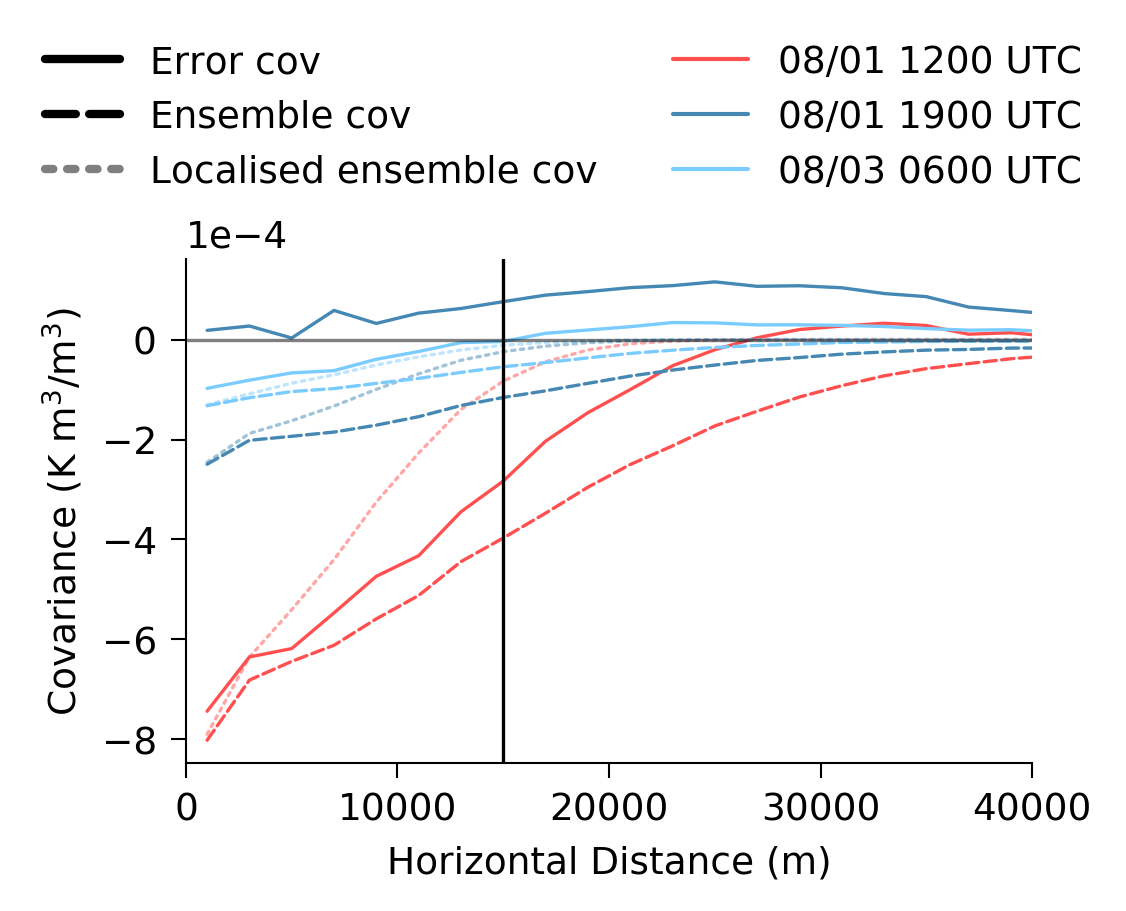
\includegraphics[width=0.48\textwidth]{figures/fig_11_covariance_dist.png}
	\caption{
		Covariances between 2-metre-temperature and soil moisture in root-depth as function of the distance between observation and grid point for the LETKF Soil+Temp experiment.
		The error covariances are estimated based on the ensemble mean errors with the covariance statistics estimated over the corresponding bin.s
		The ensemble covariances are a binned mean of the ensemble covariances, whereas the covariances are multiplied by the localization factor for the localized ensemble gain.
		The covariances are estimated based on randomly sampled $2000000$ pairs of grid points.
	}
	\label{fig:covariance_dist}
\end{figure}

As previously stated, we have negative error covariances during day-time, whereas we have slightly positive error covariances in the evening and night.
The ensemble covariances at 2015-08-01 12:00Z and 2015-08-03 06:00Z resemble the error covariances for local areas.
Nevertheless, the ensemble covariances show in both cases too wide horizontal covariances compared to the error covariances, and here, horizontal localization helps to reduce the impact of these spurious correlations.
The chosen localization radius of $15\,\text{km}$ is too small for 2015-08-01 12:00Z and reduces the impact of horizontal covariances too strongly compared to the error covariances, whereas the radius is well-tuned for 2015-08-03 06:00Z.
At 2015-08-01 19:00Z, the ensemble cannot represent the positive error covariances, and we would expect a negative assimilation impact.
In this case, the best localization would be $0\,\text{km}$, indicating that a deactivation of the assimilation would be the best choice.
The correct localization radius for cross-compartmental data assimilation is therefore highly dependent on the governing processes.

\section{Discussion and Summary}

In this study, we investigate how we can use an Ensemble Kalman filter (EnKF) to assimilate sparse 2-metre-temperature observations across the atmosphere-land interface.
Because we focus on the coupling between temperature in the atmospheric boundary layer and soil moisture, we perturb only initial soil conditions to generate an ensemble of forecasts.
All resulting deviations within the ensemble and between different experiments are therefore only a consequence of these initial soil conditions or due to data assimilation.
With this idealized experimentation framework, we are able to prove that
the soil moisture analysis can be improved by assimilating boundary layer observations.

The coupling of the land surface to the boundary layer drives this positive assimilation impact during day-time, whereas we have a neutral impact at night.
An EnKF with hourly filtering can exploit this coupling, if the ensemble covariances are representative for the error covariances.
To shape the ensemble covariances, a well-tuned horizontal localization is crucial for the cross-compartmental assimilation.
In the case of representative ensemble covariances, additional updates of the boundary layer temperature increase the consistency of the analysis increments, which has an additional positive assimilation impact on subsequent soil moisture analyses.
This additional assimilation impact hints at a positive consequence of strongly-coupled data assimilation at the atmosphere-land interface.

The EnKF has smaller errors than the Simplified Extended Kalman filter (SEKF) to our NATURE run in both, the soil moisture and boundary layer temperature.
The EnKF improves hereby the soil moisture analysis by a larger amount than the boundary layer forecast compared to the SEKF.
Our offline data assimilation experiments reveal that this is related to the finite-differences' approximation within the SEKF, which can be stabilized by using ensemble-based covariances.
We further improve the soil moisture analysis with hourly-based filtering, as it is commonly used for data assimilation in the atmosphere.
This improvement by filtering indicates that we can include land surface variables in the ensemble-based analysis cycles of the atmosphere.

With a localized EnKF, we can skip the optimal interpolation step to create a 2-metre-temperature analysis.
We find with our offline data assimilation experiments that the additional assimilation impact of a fully-observed 2-metre-temperature field is small compared to the general assimilation impact with coarsely-distributed observations.
Furthermore, the additional optimal interpolation step creates uncertainties in the temperature observations, which we have not taken into account in our offline data assimilation experiment.
Three-dimensional ensemble-based data assimilation of boundary layer observations for the soil moisture is thus possible with localization.

We have a non-linear coupling between atmospheric boundary layer and land surface, because the strength of the coupling depends on the soil moisture itself.
We only make a local linear assumption around the ensemble mean in the ensemble Kalman filter, and these non-linearities do not have a large impact on the results.
The global non-linear structure nevertheless constrains the coupling between the atmosphere and land, and above very dry and humid soils, only limited information content is encoded in observations, which is extractable by direct assimilation of the observations.

Beside this dependence of the assimilation on the coupling and on the soil moisture, we also show that the temporal development of the boundary layer has an impact.
This impact leads to a peak in information content around noon, whereas we have a decrease in the afternoon.
A partial collapse of the boundary layer into a thin layer above the land surface initiates a reinforcement of the atmosphere-land coupling.
We can more easily use the temporal development with hourly-filtering, whereas we might have problems with daily-smoothing as done within the SEKF, because we would have to select representative observation times.

We can further exploit the temporal development of the boundary layer with hourly-smoothing instead of hourly-filtering.
Because land surface perturbations need some time to propagate into the atmosphere, one possibility would be to assimilate future observations within a given assimilation window and a 4D-LETKF \citep{harlim_four-dimensional_2007,kalnay_response_2007}, which would be similar to an Iterative Ensemble Kalman smoothing scheme \citep{kalnay_accelerating_2010, sakov_iterative_2012,bocquet_iterative_2014}.
Together with smoothing, we could additionally introduce time-dependent localization to tackle problems related to errors by the ensemble approximation of the covariances.

All in all, our results support the view that assimilation of boundary layer observations has a positive impact on the soil moisture, if the model system can adequately represent the governing processes in the boundary layer and land surface.
We can therefore see this study as first step towards the goal of assimilating a unified set of observations across the atmosphere-land interface to improve the analysis for both compartments.

\section{Conclusions}
In this study, we assimilate synthetic 2-metre-temperature observations into soil moisture in a fully-coupled limited-area model system for a seven-day period in Summer 2015.
Based on our results in idealized twin experiments, we conclude the following:
\begin{enumerate}
	\item Assimilation of boundary layer observations improves the soil moisture analysis during day-time and has no impact during night; boundary layer observations yield the highest information content for land surface data assimilation above soil moisture saturations between $0.2$ and $0.5$. 
	\item Hourly-updating the soil moisture with a Localized Ensemble Transform Kalman filter results in a smaller error for the soil moisture analysis than daily-smoothing with a Simplified Extended Kalman filter, and in addition, we can directly assimilate sparse boundary layer observations across the atmosphere-land interface without an intermediate optimal interpolation step.
	\item Ensemble-based approximations of the background covariances and Jacobians stabilizes the analysis increments in a Simplified Extended Kalman filter.
	\item Updating the atmospheric temperature together with the soil moisture increases the physical consistency in the analysis for the boundary layer and land surface, which in fact reduces additional errors in the soil moisture analysis.
	\item We can merge the decoupled data assimilation cycles -- one for the land surface and one for numerical weather prediction -- into one strongly-coupled cycle with updates across the atmosphere-land interface and hour-like cycling lengths of the faster atmospheric compartment.
\end{enumerate}


\codeavailability{
	Scripts used for the experiments and results can be found under \url{https://github.com/tobifinn/letkf_t2m_h2osoi}.
	We additionlly provide the source code for the coupling framework and the data assimilation under \cite{finn_py_bacy_2020, finn_torch-assimilate_2020}, whereas the modelling platform TerrSysMP can be obtained from \url{https://www.terrsysmp.org/}.
}

\authorcontribution{
	TF, GG, and FA initialized the research idea.
	TF constructed the experiments and scripts for the results, whereas the results were discussed by TF, GG, and FA.
	TF composed the initial manuscript, which was refined by TF, GG, and FA.
}

\competinginterests{
	The authors declare that they have no conflict of interest.
}

\begin{acknowledgements}
	This work is a contribution to the project FOR2131, "Data Assimilation for Improved Characterization of Fluxes across Compartmental Interfaces", funded by the
	"Deutsche Forschungsgemeinschaft" (DFG, German Research
	Foundation) under grant 243358811.
	We would thank the whole research unit FOR2131 for discussions along the track and especially Bernd Schalge for providing us the data for the initial spin-up and lateral boundary conditions.
	In addition, we want to acknowledge researchers at the "Deutscher Wetterdienst" for helpful hints in the initial phase of the research.
\end{acknowledgements}

\bibliographystyle{copernicus}
\bibliography{19_soil_assimilation}


\end{document}




